%%
% Copyright (c) 2017 - 2021, Pascal Wagler;
% Copyright (c) 2014 - 2021, John MacFarlane
%
% All rights reserved.
%
% Redistribution and use in source and binary forms, with or without
% modification, are permitted provided that the following conditions
% are met:
%
% - Redistributions of source code must retain the above copyright
% notice, this list of conditions and the following disclaimer.
%
% - Redistributions in binary form must reproduce the above copyright
% notice, this list of conditions and the following disclaimer in the
% documentation and/or other materials provided with the distribution.
%
% - Neither the name of John MacFarlane nor the names of other
% contributors may be used to endorse or promote products derived
% from this software without specific prior written permission.
%
% THIS SOFTWARE IS PROVIDED BY THE COPYRIGHT HOLDERS AND CONTRIBUTORS
% "AS IS" AND ANY EXPRESS OR IMPLIED WARRANTIES, INCLUDING, BUT NOT
% LIMITED TO, THE IMPLIED WARRANTIES OF MERCHANTABILITY AND FITNESS
% FOR A PARTICULAR PURPOSE ARE DISCLAIMED. IN NO EVENT SHALL THE
% COPYRIGHT OWNER OR CONTRIBUTORS BE LIABLE FOR ANY DIRECT, INDIRECT,
% INCIDENTAL, SPECIAL, EXEMPLARY, OR CONSEQUENTIAL DAMAGES (INCLUDING,
% BUT NOT LIMITED TO, PROCUREMENT OF SUBSTITUTE GOODS OR SERVICES;
% LOSS OF USE, DATA, OR PROFITS; OR BUSINESS INTERRUPTION) HOWEVER
% CAUSED AND ON ANY THEORY OF LIABILITY, WHETHER IN CONTRACT, STRICT
% LIABILITY, OR TORT (INCLUDING NEGLIGENCE OR OTHERWISE) ARISING IN
% ANY WAY OUT OF THE USE OF THIS SOFTWARE, EVEN IF ADVISED OF THE
% POSSIBILITY OF SUCH DAMAGE.
%%

%%
% This is the Eisvogel pandoc LaTeX template.
%
% For usage information and examples visit the official GitHub page:
% https://github.com/Wandmalfarbe/pandoc-latex-template
%%

% Options for packages loaded elsewhere
\PassOptionsToPackage{unicode}{hyperref}
\PassOptionsToPackage{hyphens}{url}
\PassOptionsToPackage{dvipsnames,svgnames*,x11names*,table}{xcolor}
%
\documentclass[
  english,
  paper=a4,
  oneside  ,captions=tableheading
]{scrbook}
\usepackage{amsmath,amssymb}
\usepackage{lmodern}
\usepackage{setspace}
\setstretch{1.2}
\usepackage{ifxetex,ifluatex}
\ifnum 0\ifxetex 1\fi\ifluatex 1\fi=0 % if pdftex
  \usepackage[T1]{fontenc}
  \usepackage[utf8]{inputenc}
  \usepackage{textcomp} % provide euro and other symbols
\else % if luatex or xetex
  \usepackage{unicode-math}
  \defaultfontfeatures{Scale=MatchLowercase}
  \defaultfontfeatures[\rmfamily]{Ligatures=TeX,Scale=1}
\fi
% Use upquote if available, for straight quotes in verbatim environments
\IfFileExists{upquote.sty}{\usepackage{upquote}}{}
\IfFileExists{microtype.sty}{% use microtype if available
  \usepackage[]{microtype}
  \UseMicrotypeSet[protrusion]{basicmath} % disable protrusion for tt fonts
}{}
\makeatletter
\@ifundefined{KOMAClassName}{% if non-KOMA class
  \IfFileExists{parskip.sty}{%
    \usepackage{parskip}
  }{% else
    \setlength{\parindent}{0pt}
    \setlength{\parskip}{6pt plus 2pt minus 1pt}}
}{% if KOMA class
  \KOMAoptions{parskip=half}}
\makeatother
\usepackage{fancyvrb}
\usepackage{xcolor}
\definecolor{default-linkcolor}{HTML}{A50000}
\definecolor{default-filecolor}{HTML}{A50000}
\definecolor{default-citecolor}{HTML}{4077C0}
\definecolor{default-urlcolor}{HTML}{4077C0}
\IfFileExists{xurl.sty}{\usepackage{xurl}}{} % add URL line breaks if available
\IfFileExists{bookmark.sty}{\usepackage{bookmark}}{\usepackage{hyperref}}
\hypersetup{
  pdftitle={Project Requirements, Plan and Task Definitions},
  pdfauthor={Callum Stewart; Saad Badshah; Abigail Rivera; Daniel Scott; Bruce Wilson; Sebastian Zebrowski},
  pdflang={en},
  hidelinks,
  breaklinks=true,
  pdfcreator={LaTeX via pandoc with the Eisvogel template}}
\urlstyle{same} % disable monospaced font for URLs
\VerbatimFootnotes % allow verbatim text in footnotes
\usepackage[margin=2.5cm,includehead=true,includefoot=true,centering,]{geometry}
\usepackage{listings}
\newcommand{\passthrough}[1]{#1}
\lstset{defaultdialect=[5.3]Lua}
\lstset{defaultdialect=[x86masm]Assembler}
\usepackage{longtable,booktabs,array}
\usepackage{calc} % for calculating minipage widths
% Correct order of tables after \paragraph or \subparagraph
\usepackage{etoolbox}
\makeatletter
\patchcmd\longtable{\par}{\if@noskipsec\mbox{}\fi\par}{}{}
\makeatother
% Allow footnotes in longtable head/foot
\IfFileExists{footnotehyper.sty}{\usepackage{footnotehyper}}{\usepackage{footnote}}
\makesavenoteenv{longtable}
% add backlinks to footnote references, cf. https://tex.stackexchange.com/questions/302266/make-footnote-clickable-both-ways
\usepackage{footnotebackref}
\usepackage{graphicx}
\makeatletter
\def\maxwidth{\ifdim\Gin@nat@width>\linewidth\linewidth\else\Gin@nat@width\fi}
\def\maxheight{\ifdim\Gin@nat@height>\textheight\textheight\else\Gin@nat@height\fi}
\makeatother
% Scale images if necessary, so that they will not overflow the page
% margins by default, and it is still possible to overwrite the defaults
% using explicit options in \includegraphics[width, height, ...]{}
\setkeys{Gin}{width=\maxwidth,height=\maxheight,keepaspectratio}
% Set default figure placement to htbp
\makeatletter
\def\fps@figure{htbp}
\makeatother
\setlength{\emergencystretch}{3em} % prevent overfull lines
\providecommand{\tightlist}{%
  \setlength{\itemsep}{0pt}\setlength{\parskip}{0pt}}
\setcounter{secnumdepth}{-\maxdimen} % remove section numbering

% Make use of float-package and set default placement for figures to H.
% The option H means 'PUT IT HERE' (as  opposed to the standard h option which means 'You may put it here if you like').
\usepackage{float}
\floatplacement{figure}{H}

\ifxetex
    % See issue https://github.com/reutenauer/polyglossia/issues/127
  \renewcommand*\familydefault{\sfdefault}
    % Load polyglossia as late as possible: uses bidi with RTL langages (e.g. Hebrew, Arabic)
  \usepackage{polyglossia}
  \setmainlanguage[]{}
\else
  \usepackage[main=english]{babel}
% get rid of language-specific shorthands (see #6817):
\let\LanguageShortHands\languageshorthands
\def\languageshorthands#1{}
\fi
\ifluatex
  \usepackage{selnolig}  % disable illegal ligatures
\fi

\title{Project Requirements, Plan and Task Definitions}
\usepackage{etoolbox}
\makeatletter
\providecommand{\subtitle}[1]{% add subtitle to \maketitle
  \apptocmd{\@title}{\par {\large #1 \par}}{}{}
}
\makeatother
\subtitle{Deliverable 1 Report}
\author{Callum Stewart \and Saad Badshah \and Abigail Rivera \and Daniel
Scott \and Bruce Wilson \and Sebastian Zebrowski}
\date{2021-01-31}



%%
%% added
%%

%
% language specification
%
% If no language is specified, use English as the default main document language.
%



%
% for the background color of the title page
%
\usepackage{pagecolor}
\usepackage{afterpage}
\usepackage[margin=2.5cm,includehead=true,includefoot=true,centering]{geometry}

%
% break urls
%
\PassOptionsToPackage{hyphens}{url}

%
% When using babel or polyglossia with biblatex, loading csquotes is recommended
% to ensure that quoted texts are typeset according to the rules of your main language.
%
\usepackage{csquotes}

%
% captions
%
\definecolor{caption-color}{HTML}{777777}
\usepackage[font={stretch=1.2}, textfont={color=caption-color}, position=top, skip=4mm, labelfont=bf, singlelinecheck=false, justification=raggedright]{caption}
\setcapindent{0em}

%
% blockquote
%
\definecolor{blockquote-border}{RGB}{221,221,221}
\definecolor{blockquote-text}{RGB}{119,119,119}
\usepackage{mdframed}
\newmdenv[rightline=false,bottomline=false,topline=false,linewidth=3pt,linecolor=blockquote-border,skipabove=\parskip]{customblockquote}
\renewenvironment{quote}{\begin{customblockquote}\list{}{\rightmargin=0em\leftmargin=0em}%
\item\relax\color{blockquote-text}\ignorespaces}{\unskip\unskip\endlist\end{customblockquote}}

%
% Source Sans Pro as the de­fault font fam­ily
% Source Code Pro for monospace text
%
% 'default' option sets the default
% font family to Source Sans Pro, not \sfdefault.
%
\ifnum 0\ifxetex 1\fi\ifluatex 1\fi=0 % if pdftex
    \usepackage[default]{sourcesanspro}
  \usepackage{sourcecodepro}
  \else % if not pdftex
    \usepackage[default]{sourcesanspro}
  \usepackage{sourcecodepro}

  % XeLaTeX specific adjustments for straight quotes: https://tex.stackexchange.com/a/354887
  % This issue is already fixed (see https://github.com/silkeh/latex-sourcecodepro/pull/5) but the
  % fix is still unreleased.
  % TODO: Remove this workaround when the new version of sourcecodepro is released on CTAN.
  \ifxetex
    \makeatletter
    \defaultfontfeatures[\ttfamily]
      { Numbers   = \sourcecodepro@figurestyle,
        Scale     = \SourceCodePro@scale,
        Extension = .otf }
    \setmonofont
      [ UprightFont    = *-\sourcecodepro@regstyle,
        ItalicFont     = *-\sourcecodepro@regstyle It,
        BoldFont       = *-\sourcecodepro@boldstyle,
        BoldItalicFont = *-\sourcecodepro@boldstyle It ]
      {SourceCodePro}
    \makeatother
  \fi
  \fi

%
% heading color
%
\definecolor{heading-color}{RGB}{40,40,40}
\addtokomafont{section}{\color{heading-color}}
% When using the classes report, scrreprt, book,
% scrbook or memoir, uncomment the following line.
%\addtokomafont{chapter}{\color{heading-color}}

%
% variables for title, author and date
%
\usepackage{titling}
\title{Project Requirements, Plan and Task Definitions}
\author{Callum Stewart, Saad Badshah, Abigail Rivera, Daniel
Scott, Bruce Wilson, Sebastian Zebrowski}
\date{2021-01-31}

%
% tables
%

\definecolor{table-row-color}{HTML}{F5F5F5}
\definecolor{table-rule-color}{HTML}{999999}

%\arrayrulecolor{black!40}
\arrayrulecolor{table-rule-color}     % color of \toprule, \midrule, \bottomrule
\setlength\heavyrulewidth{0.3ex}      % thickness of \toprule, \bottomrule
\renewcommand{\arraystretch}{1.3}     % spacing (padding)


%
% remove paragraph indention
%
\setlength{\parindent}{0pt}
\setlength{\parskip}{6pt plus 2pt minus 1pt}
\setlength{\emergencystretch}{3em}  % prevent overfull lines

%
%
% Listings
%
%


%
% general listing colors
%
\definecolor{listing-background}{HTML}{F7F7F7}
\definecolor{listing-rule}{HTML}{B3B2B3}
\definecolor{listing-numbers}{HTML}{B3B2B3}
\definecolor{listing-text-color}{HTML}{000000}
\definecolor{listing-keyword}{HTML}{435489}
\definecolor{listing-keyword-2}{HTML}{1284CA} % additional keywords
\definecolor{listing-keyword-3}{HTML}{9137CB} % additional keywords
\definecolor{listing-identifier}{HTML}{435489}
\definecolor{listing-string}{HTML}{00999A}
\definecolor{listing-comment}{HTML}{8E8E8E}

\lstdefinestyle{eisvogel_listing_style}{
  language         = java,
  numbers          = left,
  xleftmargin      = 2.7em,
  framexleftmargin = 2.5em,
  backgroundcolor  = \color{listing-background},
  basicstyle       = \color{listing-text-color}\linespread{1.0}\scriptsize\ttfamily{},
  breaklines       = true,
  frame            = single,
  framesep         = 0.19em,
  rulecolor        = \color{listing-rule},
  frameround       = ffff,
  tabsize          = 4,
  numberstyle      = \color{listing-numbers},
  aboveskip        = 1.0em,
  belowskip        = 0.1em,
  abovecaptionskip = 0em,
  belowcaptionskip = 1.0em,
  keywordstyle     = {\color{listing-keyword}\bfseries},
  keywordstyle     = {[2]\color{listing-keyword-2}\bfseries},
  keywordstyle     = {[3]\color{listing-keyword-3}\bfseries\itshape},
  sensitive        = true,
  identifierstyle  = \color{listing-identifier},
  commentstyle     = \color{listing-comment},
  stringstyle      = \color{listing-string},
  showstringspaces = false,
  escapeinside     = {/*@}{@*/}, % Allow LaTeX inside these special comments
  literate         =
  {á}{{\'a}}1 {é}{{\'e}}1 {í}{{\'i}}1 {ó}{{\'o}}1 {ú}{{\'u}}1
  {Á}{{\'A}}1 {É}{{\'E}}1 {Í}{{\'I}}1 {Ó}{{\'O}}1 {Ú}{{\'U}}1
  {à}{{\`a}}1 {è}{{\'e}}1 {ì}{{\`i}}1 {ò}{{\`o}}1 {ù}{{\`u}}1
  {À}{{\`A}}1 {È}{{\'E}}1 {Ì}{{\`I}}1 {Ò}{{\`O}}1 {Ù}{{\`U}}1
  {ä}{{\"a}}1 {ë}{{\"e}}1 {ï}{{\"i}}1 {ö}{{\"o}}1 {ü}{{\"u}}1
  {Ä}{{\"A}}1 {Ë}{{\"E}}1 {Ï}{{\"I}}1 {Ö}{{\"O}}1 {Ü}{{\"U}}1
  {â}{{\^a}}1 {ê}{{\^e}}1 {î}{{\^i}}1 {ô}{{\^o}}1 {û}{{\^u}}1
  {Â}{{\^A}}1 {Ê}{{\^E}}1 {Î}{{\^I}}1 {Ô}{{\^O}}1 {Û}{{\^U}}1
  {œ}{{\oe}}1 {Œ}{{\OE}}1 {æ}{{\ae}}1 {Æ}{{\AE}}1 {ß}{{\ss}}1
  {ç}{{\c c}}1 {Ç}{{\c C}}1 {ø}{{\o}}1 {å}{{\r a}}1 {Å}{{\r A}}1
  {€}{{\EUR}}1 {£}{{\pounds}}1 {«}{{\guillemotleft}}1
  {»}{{\guillemotright}}1 {ñ}{{\~n}}1 {Ñ}{{\~N}}1 {¿}{{?`}}1
  {…}{{\ldots}}1 {≥}{{>=}}1 {≤}{{<=}}1 {„}{{\glqq}}1 {“}{{\grqq}}1
  {”}{{''}}1
}
\lstset{style=eisvogel_listing_style}

%
% Java (Java SE 12, 2019-06-22)
%
\lstdefinelanguage{Java}{
  morekeywords={
    % normal keywords (without data types)
    abstract,assert,break,case,catch,class,continue,default,
    do,else,enum,exports,extends,final,finally,for,if,implements,
    import,instanceof,interface,module,native,new,package,private,
    protected,public,requires,return,static,strictfp,super,switch,
    synchronized,this,throw,throws,transient,try,volatile,while,
    % var is an identifier
    var
  },
  morekeywords={[2] % data types
    % primitive data types
    boolean,byte,char,double,float,int,long,short,
    % String
    String,
    % primitive wrapper types
    Boolean,Byte,Character,Double,Float,Integer,Long,Short
    % number types
    Number,AtomicInteger,AtomicLong,BigDecimal,BigInteger,DoubleAccumulator,DoubleAdder,LongAccumulator,LongAdder,Short,
    % other
    Object,Void,void
  },
  morekeywords={[3] % literals
    % reserved words for literal values
    null,true,false,
  },
  sensitive,
  morecomment  = [l]//,
  morecomment  = [s]{/*}{*/},
  morecomment  = [s]{/**}{*/},
  morestring   = [b]",
  morestring   = [b]',
}

\lstdefinelanguage{XML}{
  morestring      = [b]",
  moredelim       = [s][\bfseries\color{listing-keyword}]{<}{\ },
  moredelim       = [s][\bfseries\color{listing-keyword}]{</}{>},
  moredelim       = [l][\bfseries\color{listing-keyword}]{/>},
  moredelim       = [l][\bfseries\color{listing-keyword}]{>},
  morecomment     = [s]{<?}{?>},
  morecomment     = [s]{<!--}{-->},
  commentstyle    = \color{listing-comment},
  stringstyle     = \color{listing-string},
  identifierstyle = \color{listing-identifier}
}

%
% header and footer
%
\usepackage{fancyhdr}

\fancypagestyle{eisvogel-header-footer}{
  \fancyhead{}
  \fancyfoot{}
  \lhead[2021-01-31]{Project Requirements, Plan and Task Definitions}
  \chead[]{}
  \rhead[Project Requirements, Plan and Task Definitions]{2021-01-31}
  \lfoot[\thepage]{Callum Stewart, Saad Badshah, Abigail Rivera, Daniel
Scott, Bruce Wilson, Sebastian Zebrowski}
  \cfoot[]{}
  \rfoot[Callum Stewart, Saad Badshah, Abigail Rivera, Daniel
Scott, Bruce Wilson, Sebastian Zebrowski]{\thepage}
  \renewcommand{\headrulewidth}{0.4pt}
  \renewcommand{\footrulewidth}{0.4pt}
}
\pagestyle{eisvogel-header-footer}

%%
%% end added
%%

\begin{document}

%%
%% begin titlepage
%%
\begin{titlepage}
\newgeometry{left=6cm}
\definecolor{titlepage-color}{HTML}{483D8B}
\newpagecolor{titlepage-color}\afterpage{\restorepagecolor}
\newcommand{\colorRule}[3][black]{\textcolor[HTML]{#1}{\rule{#2}{#3}}}
\begin{flushleft}
\noindent
\\[-1em]
\color[HTML]{FFFAFA}
\makebox[0pt][l]{\colorRule[FFFAFA]{1.3\textwidth}{2pt}}
\par
\noindent

{
  \setstretch{1.4}
  \vfill
  \noindent {\huge \textbf{\textsf{Project Requirements, Plan and Task
Definitions}}}
    \vskip 1em
  {\Large \textsf{Deliverable 1 Report}}
    \vskip 2em
  \noindent {\Large \textsf{Callum Stewart, Saad Badshah, Abigail
Rivera, Daniel Scott, Bruce Wilson, Sebastian Zebrowski}}
  \vfill
}


\textsf{2021-01-31}
\end{flushleft}
\end{titlepage}
\restoregeometry

%%
%% end titlepage
%%


\tableofcontents
\newpage

\hypertarget{background-and-motivation}{%
\section{Background and Motivation}\label{background-and-motivation}}

\hypertarget{motivation}{%
\subsection{Motivation}\label{motivation}}

In this project we are seeking to create an educational tool that can be
used to interactively explore the differences between two approaches to
time series analysis of non-stationary signals. The front end only
application will allow users to either submit their own signals, or to
build one using a library of predefined signal types, and then perform
either a Short Time Fourier Transform or a Empirical Mode Decomposition
on the signal to break it down into it's constituent component signals.

This will allow them to explore the differences between these two
methods for decomposing time signals, serving as a demonstration of
their relative strengths and weakness, and providing an intuitive feel
for how they work. The application will also have a number of
convenience features for users, such as the ability to bookmark
examples, and a pre-generated set of examples that can be used to
demonstrate how the application and how the time series analysis
techniques work.

\hypertarget{background}{%
\subsection{Background}\label{background}}

\hypertarget{time-series-analysis}{%
\subsubsection{Time Series Analysis}\label{time-series-analysis}}

A \emph{time series} is a sequence of data points that are indexed or
graphed in time order. Frequently graphed in a run chart (a graph which
features time as its \(y\) axis), time series occur naturally in a
wide array of subjects, such as statistics, finance, weather
forecasting, and signal processing.

There are a handful of common types of time series that occur widely,
for example: 

\begin{enumerate}
	\item Simple sinusoids 
	\item Linear, exponential, logarithmic, or polynomial trends 
	\item White, coloured, or shot noise 
	\item Chirps 
	\item Products and sums of the above signals, forming complex signals that might be found in the real world
\end{enumerate}

\emph{Time series analysis} is a set of techniques that can be used in
order to reason about time series', enabling an analyst to extract
useful insights from the data.

Many time series exhibit an oscillatory behaviour, such as the
temperature of a city on any given day of the year, the share price of a
given stock, or the audio data recorded by a microphone. An analyst can
exploit the fact that complex signals can be approximated with sums of
simpler trigonometric functions and use Fourier analysis to decompose a
signal into its oscillatory components.

\hypertarget{discrete-fourier-transform}{%
\subsubsection{Discrete Fourier
Transform}\label{discrete-fourier-transform}}

\begin{figure}
\centering
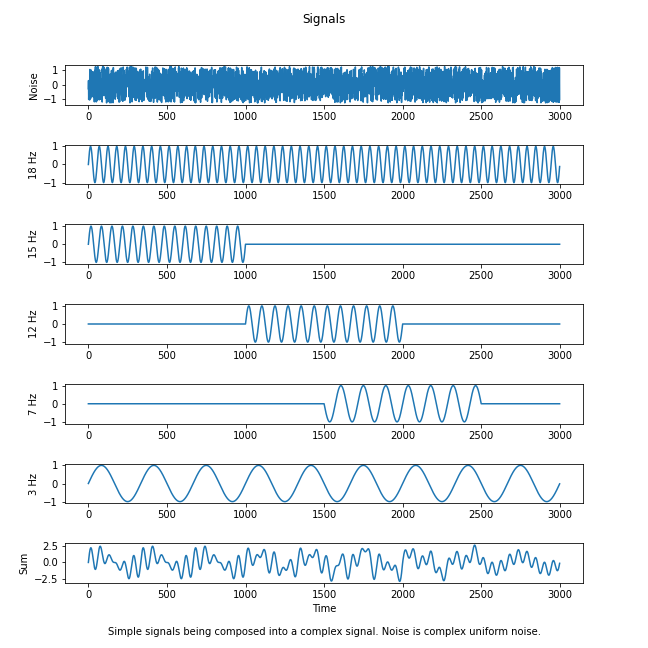
\includegraphics{img/composite_signal.png}
\caption{Complex signal derived from simple signals}
\end{figure}

A Fourier transform is one way of decomposing a complex signal into its
oscillatory components, revealing the frequencies of the constituent
component signals. Determining what component frequencies are present in
a signal can give an insight into the nature of a signal, or allow it to
be manipulated precisely. For example, it may allow an audio engineer to
silence or boost particular frequencies as they see fit, or a financial
analyst to determine what kind of long term trends exist in financial
data. Lets look at an example of a Fourier transform of the previous
signal. We will use the Fast Fourier Transform (FFT) algorithm to
compute the transform.

\begin{figure}
\centering
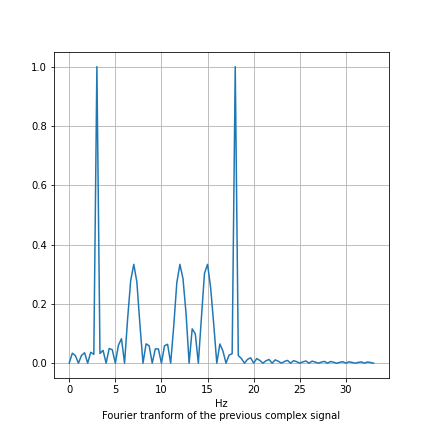
\includegraphics{img/fft.png}
\caption{Fourier transform of complex signal}
\end{figure}

Notice that despite having a strong indication that the constant 3Hz and
18Hz signals are constituent components, much information has been lost.
As a Fourier transform maps a function from the time domain to the
frequency domain, all temporal information is lost, as the FFT assumes
periodicity. This is obviously not ideal, as our complex signal is
non-linear. The Fourier transform is thus not well suited to non-linear
signals when applied on the entire signal at once.

\hypertarget{short-time-fourier-transform}{%
\subsubsection{Short Time Fourier
Transform}\label{short-time-fourier-transform}}

Instead, in order to study non-stationary signals, we require a
technique that can study a signal in both the time and frequency domain
simultaneously. The simplest of these techniques is the Short Time
Fourier Transform (STFT).

The procedure for STFT is to divide a long time signal equally into
shorter length segments, and then compute a DFT on each of these
segments. In order to smooth out any unusual artefacts at the boundary
of segments, window functions such as a Hann window may be used, which
attenuates signals located near boundaries using a cosine window. With
the Fourier spectra of each shorter segment, we can plot the changing
spectra against time using a type of plot known as a spectrogram. Here
is an example of STFT applied to our original signal.

\begin{figure}
\centering
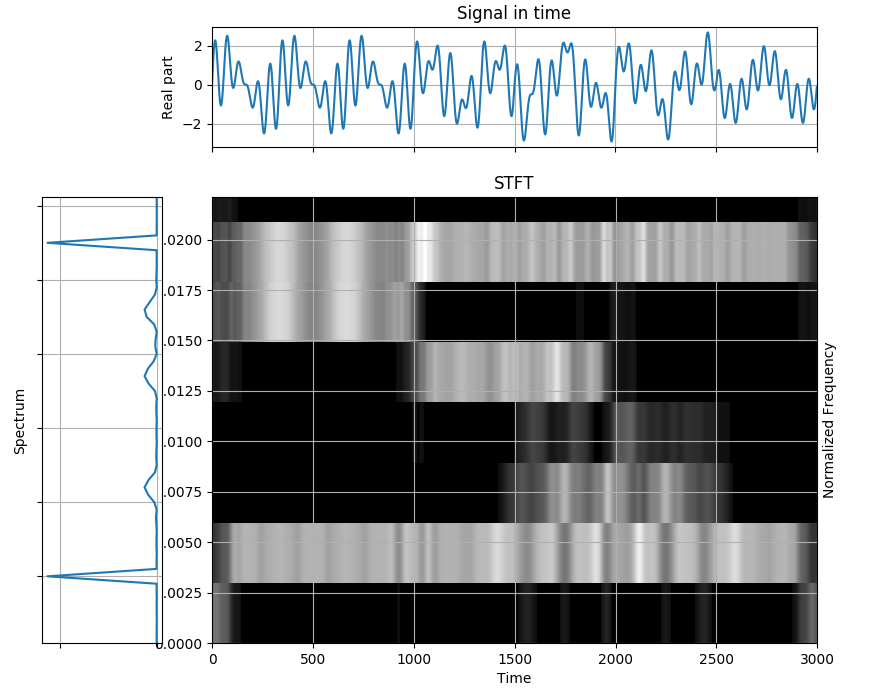
\includegraphics{img/stft_output_spectra.png}
\caption{Resulting spectra from STFT applied to complex signal}
\end{figure}

Here we can see the strength of each constituent signal by colour
intensity. Unlike previously with the FFT, we now have temporal
information, and can see when signals of a given frequency begin and end
in the complex signal.

However there is a significant limitation to building on top of Fourier
transforms due to an uncertainty limit called the Gabor limit. By making
the time resolution smaller (i.e., by dividing the main signal into
smaller windows) we become more certain of when frequencies change, but
we lose frequency resolution (the ability to see frequency components
close together). By making the time resolutions larger, we lose time
resolution (the ability to know precisely when a frequency changes), but
we get better frequency resolution.

\hypertarget{hilbert-huang-transform-and-empirical-mode-decomposition}{%
\subsubsection{Hilbert-Huang Transform and Empirical Mode
Decomposition}\label{hilbert-huang-transform-and-empirical-mode-decomposition}}

The Hilbert-Huang Transform (HHT) is a powerful time-frequency analysis
technique. It allows an analyst to decompose a complex signal into a
number of orthogonal Intrinsic Mode Frequencies (IMFs) with a trend
using EMD and applies Hilbert Spectral Analysis (HSA) to the IMFs to
obtain information regarding instantaneous frequency.

HHT first utilises empirical mode decomposition (EMD) in order to break
a complex waveform into IMFs representing simple oscillatory modes
through a process called sifting. The amplitude and frequency of an IMF
may vary with time, and must satisfy both of these rules: 

\begin{enumerate}
	\item The total number of extrema and the number of zero crossings must differ by at most 1 
	\item The mean envelope value (defined by a spline described by the local maxima and the local minima) must be nearly zero
\end{enumerate}

The sifting procedure to extract these IMFs can be described by the following steps: 

\begin{enumerate}
	\item Initialise \(r_0 = X(t)\) and \(i = 1\)
	\item Start outer loop 
	\item Extract the \(i\)th IMF \(c_i\)
	\begin{enumerate}
		\item Initialise \(h_{k(k-1)} = r_{i-1}\), \(k = 1\)
		\item Start inner loop
		\item Identify all of the local maxima and minima (the extrema)
		\item Interpolate the minima with a cubic spline in order to define the lower envelope
		\item Interpolate the maxima with a cubic spline in order to define the upper envelope
		\item Calculate the mean \(m_{i(k-1)}\) of the upper and lower envelopes of \(h_{i(k-1)}\). The envelope defined by the two cubic splines should contain all data.
		\item Set \(h_{ik} = h_{i(k-1)} - m_{i(k-1)}\)
		\item Is \(h_{ik}\) an IMF? 
		\begin{itemize}
			\item If true, set \(c_i = h_{ik}\) and break 
			\item Else increment \(k\) and continue inner loop
		\end{itemize}
	\end{enumerate}
	\item Set the remainder \(r_{i+1} = r_i - c_i\)
	\item Does \(r_{i + 1}\) contain at least two extrema?
	\begin{itemize}
		\item If true increment \(i\) and continue outer loop
		\item Else end routine, with \(r_{i + 1}\) as the signal residue and \(c_1\) through \(c_i\) as the IMFs
	\end{itemize}
\end{enumerate}

Below is a flowchart describing this algorithm\footnote{Lei, Yaguo, et
  al.~``A review on empirical mode decomposition in fault diagnosis of
  rotating machinery.'' \emph{Mechanical systems and signal processing
  35.1-2} (2013): 108-126.}

\begin{figure}
\centering
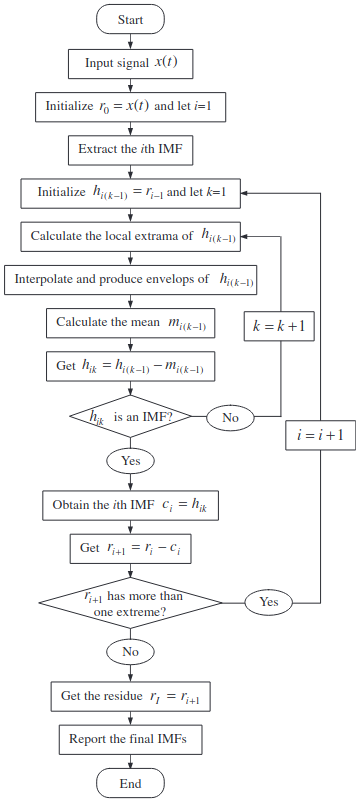
\includegraphics{img/emd_flowchart.png}
\caption{Flowchart of EMD algorithm}
\end{figure}


The number of sifting steps required to produce an IMF is determined by
the stopping criterion. There are a number of stopping criterion that
can be used for EMD, each with their own advantages and disadvantages.
The one proposed by Huang et al.~(1998) however is the `Standard
Deviation' method. For each point in time, the difference between the
current component and the previous component is calculated, squared,
divided by the square of the previous component evaluated at that point
in time, and summed.

\begin{equation}
SD_{k}=\sum _{{t=0}}^{{T}}{\frac  {|h_{{k-1}}(t)-h_{k}(t)|^{2}}{h_{{k-1}}^{2}(t)}}
\end{equation}

Once this value falls below a predetermined threshold, the sifting
process can be stopped.

There are other stopping criterion that may be used however, such as S
Number Criterion or Energy Difference Tracking.

Below we can see an example of EMD being performed on a complex signal,
breaking it down into its constituent modes in descending frequency
order\footnote{Example adapted from the Jupyter Notebook tutorials
  created by the developers of Python's \passthrough{\lstinline!emd!}
  library, available
  \href{https://emd.readthedocs.io/en/stable/_downloads/e47aacca40568b7bb056bd96535966c4/emd_tutorials_jupyter.zip}{here}}.

\begin{figure}
\centering
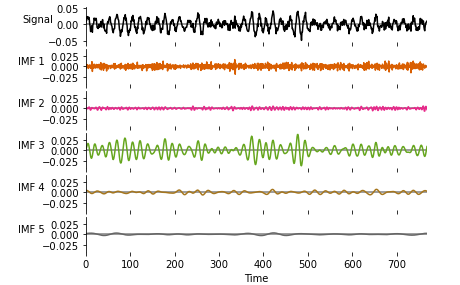
\includegraphics{img/emd_example.png}
\caption{An example of EMD being performed on a signal}
\end{figure}

At this point, if desired, the instantaneous frequency spectrum can be
obtained by applying the Hilbert transform on the constituent IMFs. The
final result would be called a Hilbert spectrum, where the amplitude and
instantaneous frequency can be plotted as functions of time on a three
dimensional plot.

Unlike STFT, EMD is a self-adaptive signal processing method. The IMFs
are determined by the signal itself, and are representative of the
natural oscillatory mode embedded in the signal. Thus EMD works on the
characteristic time local time scale, rather than with predetermined
windows.

Of course, EMD has weaknesses as well, for example:

\begin{enumerate}
\def\labelenumi{\arabic{enumi}.}
\tightlist
\item
  EMD suffers from end effects
\item
  The IMFs may not be orthogonal
\item
  Mode mixing sometimes occurs between IMFs, where a single IMF includes
  oscillatory modes that are drastically different or a component of a
  different IMF all together.
\end{enumerate}

In conclusion, each time-frequency analysis technique has draw backs and
advantages, and neither one is conclusively the correct one to use in
any given situation. This being said, for analysing non-stationary
signals EMD has some obvious advantages compared to STFT and can be
considered superior in most cases \footnote{Arun Raj P.D., Mr.~Venkatesh
  S., ``Time-Frequency Analysis methods: A Comparative study'',
  International Research Journal of Engineering and Technology
  (IRJET),Volume 3, Issue 6, June 2016, e-ISSN: 2395-0056.}.

\newpage
\hypertarget{requirements-analysis}{%
\section{Requirements Analysis}\label{requirements-analysis}}

This section of the deliverable documents and details both the
functional and constraint requirements of the application system which
are expected to be delivered in the final submission. For clarity, a
`functional' requirement refers to a component of the system which has
been explicitly specified as a necessary piece of functionality for the
system to be considered complete, whilst a `constraint' requirement can
be considered more like a non-behavioural requirement, for example the
security or portability of a given system.

Both the functional and constraint requirements have been ordered
according to the
\href{https://www.agilebusiness.org/page/ProjectFramework_10_MoSCoWPrioritisation}{MoSCoW
prioritization model}. This model ranks the requirements according to
their level of importance; a requirement may be prioritized as either
\textbf{M}ust have, \textbf{S}hould have, \textbf{C}ould have or
\textbf{W}ill not have. Certain abstract and/or actionable requirements
will be referenced later in this document with a detailed plan defining
how they will be achieved in the final system.

\newpage
\hypertarget{functional-requirements}{%
\subsection{Functional Requirements}\label{functional-requirements}}

\hypertarget{signal-analysis}{%
\subsubsection{Signal Analysis}\label{signal-analysis}}

\begin{longtable}[]{@{}
  >{\raggedright\arraybackslash}p{(\columnwidth - 4\tabcolsep) * \real{0.0656}}
  >{\raggedright\arraybackslash}p{(\columnwidth - 4\tabcolsep) * \real{0.8590}}
  >{\raggedright\arraybackslash}p{(\columnwidth - 4\tabcolsep) * \real{0.0754}}@{}}
\toprule
\begin{minipage}[b]{\linewidth}\raggedright
Requirement Number
\end{minipage} & \begin{minipage}[b]{\linewidth}\raggedright
Description
\end{minipage} & \begin{minipage}[b]{\linewidth}\raggedright
MoSCoW Prioritization
\end{minipage} \\
\midrule
\endhead
FR-1-1 & The application must support Short-Time Fourier Transform
(STFT) time series analysis on input signal data. & Must Have \\
FR-1-2 & The application must support Empirical Mode Decomposition (EMD)
time series analysis on input signal data and export the resultant IMFs
for use in other components of the application. & Must Have \\
FR-1-3 & The application must support the deconstruction of given,
identifiable signal data into its respective functional components. I.e.
Deconstruct periodical sinusoidal signal data via STFT and display its
extracted frequencies in a spectragram. & Must Have \\
\bottomrule
\end{longtable}

\hypertarget{user-interface}{%
\subsubsection{User Interface}\label{user-interface}}

\begin{longtable}[]{@{}
  >{\raggedright\arraybackslash}p{(\columnwidth - 4\tabcolsep) * \real{0.0778}}
  >{\raggedright\arraybackslash}p{(\columnwidth - 4\tabcolsep) * \real{0.8327}}
  >{\raggedright\arraybackslash}p{(\columnwidth - 4\tabcolsep) * \real{0.0895}}@{}}
\toprule
\begin{minipage}[b]{\linewidth}\raggedright
Requirement Number
\end{minipage} & \begin{minipage}[b]{\linewidth}\raggedright
Description
\end{minipage} & \begin{minipage}[b]{\linewidth}\raggedright
MoSCoW Prioritization
\end{minipage} \\
\midrule
\endhead
FR-2-1 & The application must plot the output of a signal analysis
request (STFT, EMD) on given input data visually in a graph embedded in
the webpage. & Must Have \\
FR 2-2 & The application must support simultaneously displaying the
original, unaltered signal data and the extracted components on a common
time base (i.e.~over a period of 10 seconds) in a graph embedded in the
webpage. & Must Have \\
FR 2-3 & The application must support simultaneously displaying the
instantaneous frequencies of the original components alongside the IMF
and STFT estimates in a graph embedded in the webpage. & Must Have \\
FR 2-4 & The application must support `bookmarking' functionality;
allowing users to share their configurations and parameters for signal
analysis. & Must Have \\
FR 2-5 & The application must explain the advantages and disadvantages
between STFT and EMD signal analysis. & Must Have \\
FR 2-6 & The application should display animations showcasing the
differences in techniques and behaviours between EMD and STFT analysis.
& Should Have \\
FR 2-7 & The application should allow the user to generate custom signal
data from a set of pre-defined types for processing. & Should Have \\
\bottomrule
\end{longtable}

\hypertarget{generic}{%
\subsubsection{Generic}\label{generic}}

\begin{longtable}[]{@{}
  >{\raggedright\arraybackslash}p{(\columnwidth - 4\tabcolsep) * \real{0.0709}}
  >{\raggedright\arraybackslash}p{(\columnwidth - 4\tabcolsep) * \real{0.8475}}
  >{\raggedright\arraybackslash}p{(\columnwidth - 4\tabcolsep) * \real{0.0816}}@{}}
\toprule
\begin{minipage}[b]{\linewidth}\raggedright
Requirement Number
\end{minipage} & \begin{minipage}[b]{\linewidth}\raggedright
Description
\end{minipage} & \begin{minipage}[b]{\linewidth}\raggedright
MoSCoW Prioritization
\end{minipage} \\
\midrule
\endhead
FR 3-1 & The application must be extensively tested via unit and
integration testing to verify individual components behave predictably
and correctly, and multiple components working in conjunction behave
reliably and deliver the expected result. & Must Have \\
FR 3-2 & The application must support raw signal data to be uploaded for
processing by an end user, and not just rely on pre-generated examples.
& Must Have \\
\bottomrule
\end{longtable}

\hypertarget{constraint-requirements}{%
\subsection{Constraint Requirements}\label{constraint-requirements}}

\hypertarget{interface}{%
\subsubsection{Interface}\label{interface}}

\begin{longtable}[]{@{}
  >{\raggedright\arraybackslash}p{(\columnwidth - 4\tabcolsep) * \real{0.0709}}
  >{\raggedright\arraybackslash}p{(\columnwidth - 4\tabcolsep) * \real{0.8475}}
  >{\raggedright\arraybackslash}p{(\columnwidth - 4\tabcolsep) * \real{0.0816}}@{}}
\toprule
\begin{minipage}[b]{\linewidth}\raggedright
Requirement Number
\end{minipage} & \begin{minipage}[b]{\linewidth}\raggedright
Description
\end{minipage} & \begin{minipage}[b]{\linewidth}\raggedright
MoSCoW Prioritization
\end{minipage} \\
\midrule
\endhead
NFR 1-1 & The web application will be easy to use for users. & Should
Have \\
NFR 1-2 & The application must have predefined signal types, which the
user can choose from through a drop-down list. & Must Have \\
NFR 1-3 & The web application will have an online tutorial embedded for
the users to see and learn about the advantages and disadvantages of EMD
and STFT. & Must Have \\
NFR 1-4 & Allow users to save data visualisations. & Must Have \\
\bottomrule
\end{longtable}

\hypertarget{performance}{%
\subsubsection{Performance}\label{performance}}

\begin{longtable}[]{@{}
  >{\raggedright\arraybackslash}p{(\columnwidth - 4\tabcolsep) * \real{0.0709}}
  >{\raggedright\arraybackslash}p{(\columnwidth - 4\tabcolsep) * \real{0.8475}}
  >{\raggedright\arraybackslash}p{(\columnwidth - 4\tabcolsep) * \real{0.0816}}@{}}
\toprule
\begin{minipage}[b]{\linewidth}\raggedright
Requirement Number
\end{minipage} & \begin{minipage}[b]{\linewidth}\raggedright
Description
\end{minipage} & \begin{minipage}[b]{\linewidth}\raggedright
MoSCoW Prioritization
\end{minipage} \\
\midrule
\endhead
NFR 2-1 & The web application will have no back-end, all of the
functionality will be implemented on the front-end. & Must Have \\
NFR 2-2 & The application will have low latency, the application will be
effiecient in regards to the overhead of the data visualisation. & Could
Have \\
NFR 2-3 & The application will allow different kinds of data input by
the user. It will support data in formats such as CSV. & Could Have \\
NFR 2-4 & The application will be efficent with the usage of the memory,
to allow smooth animations of the data visualisations and avoid memory
problems. & Should Have \\
\bottomrule
\end{longtable}

\hypertarget{flexibility}{%
\subsubsection{Flexibility}\label{flexibility}}

\begin{longtable}[]{@{}
  >{\raggedright\arraybackslash}p{(\columnwidth - 4\tabcolsep) * \real{0.0709}}
  >{\raggedright\arraybackslash}p{(\columnwidth - 4\tabcolsep) * \real{0.8475}}
  >{\raggedright\arraybackslash}p{(\columnwidth - 4\tabcolsep) * \real{0.0816}}@{}}
\toprule
\begin{minipage}[b]{\linewidth}\raggedright
Requirement Number
\end{minipage} & \begin{minipage}[b]{\linewidth}\raggedright
Description
\end{minipage} & \begin{minipage}[b]{\linewidth}\raggedright
MoSCoW Prioritization
\end{minipage} \\
\midrule
\endhead
NFR 3-1 & The web application will be compatibility across multiple
platforms (FireFox, Chrome). & Could Have \\
NFR 3-2 & The web application will be able to handle stress, it will be
stress tested to prevent any glitching or any unexpected events to
occur. & Could Have \\
NFR 3-3 & The application will not be tested or designed for use on
Mobile devices. & Will Not Have \\
\bottomrule
\end{longtable}

\newpage
\hypertarget{task-specifications}{%
\section{Task Specifications}\label{task-specifications}}

\begin{quote}
NB: In an effort to reduce repeated task requirements, the project will
emphasise the importance of the `Ownership' philosophy, in that the
developer who constructs a component is the SME (Subject Matter Expert)
of that component, and hence will be best suited for bug-fixing and
unit-testing that component. This replaces an explicit `Unit Testing'
task specification, whereby only 1 person in the project would be held
accountable for testing components they may not be familiar with. 
\end{quote}

\hypertarget{t2-identify-adopt-emd-algorithm-for-signal-analysis}{%
\subsection{T1: Source and adopt existing STFT analysis algorithm}\label{t1-identify-adopt-emd-algorithm-for-signal-analysis}}

\hypertarget{member-responsible-callum-stewart}{%
\paragraph{Member Responsible: Callum
Stewart}\label{member-responsible-callum-stewart}}

\hypertarget{time-required-estimate-5-hours}{%
\paragraph{Time Required (Estimate): 5
hours}\label{time-required-estimate-5-hours}}

\hypertarget{depends-on-t3-t6}{%
\paragraph{Depends on: T3, T6}\label{depends-on-t3-t6}}

\hypertarget{description}{%
\paragraph{Description:}\label{description}}
A core tenet of our application is the ability to perform Short Time Fourier Transform
analysis on a variety of given signal data types. We must, by taking all
reasonable steps, avoid implementing this complex algorithm from scratch
if possible, and instead adopt a compatible library so that we can
direct our efforts on providing functionality elsewhere in the
application. With the assumption that our Python-to-JavaScript
conversion efforts bear fruit, the
\href{https://docs.scipy.org/doc/scipy/reference/generated/scipy.signal.stft.html}{following library} may be of use.

Once a library has been deemed suitable and compatible with the
application architecture, it must be tested before adoption to verify
there are no logical inconsistencies between itself and the demo
provided to us via Cole's Jupyter notebook, which will act as our
benchmark and reference for comparisons. To speed up this process, the
proposed test plan is to compare the results of the STFT analysis
algorithm in Cole's Jupyter notebook with those returned by the library
under test. This test should then identify any logical discrepancies
between the two implementations of the algorithm: if the output does not
match exactly, the results must be investigated to identify the severity
of the difference; if it is merely a matter of accuracy (i.e.~length of
float result) then this will be noted, however if this not the case then
a deeper analysis between the two implementations will be required.

Once a library has been adopted, unit tests will then be written to
ensure consistent results consistent, reliable results are achieved
throughout development. These unit tests may then form the basis for
integration tests towards the end of development to ensure the analysis
and graphing of the results works as expected.

A breakdown of the STFT analysis can be found in the Background and
Motivation section.

\newpage
\hypertarget{t2-identify-adopt-emd-algorithm-for-signal-analysis}{%
\subsection{T2: Identify \& Adopt EMD Algorithm for Signal
Analysis}\label{t2-identify-adopt-emd-algorithm-for-signal-analysis-asdf}}

\hypertarget{member-responsible-callum-stewart}{%
\paragraph{Member Responsible: Callum
Stewart}\label{member-responsible-callum-stewart}}

\hypertarget{time-required-estimate-5-hours}{%
\paragraph{Time Required (Estimate): 5
hours}\label{time-required-estimate-5-hours-asdf}}

\hypertarget{depends-on-t3-t6}{%
\paragraph{Depends on: T3, T6}\label{depends-on-t3-t6-asdf}}

\hypertarget{description}{%
\paragraph{Description:}\label{description-asdf}}

Another tenet of this application will be its ability to perform
Empirical Mode Decomposition analysis on a given sample of signal data.
As a consequence of it being a more niche, less well-known algorithm,
priority will be assigned to this task to ensure ample time to locate a
suitable pre-existing library (for instance,
\href{https://emd.readthedocs.io/en/stable/}{this one}) and/or consult
the project stakeholders for sample code and resources to re-implement
the algorithm independently. The latter being the less desirable of the
two options due to the extra time required to ensure the robustness of
the implementation; with a `stable' release of a 3rd party library, a
reasonable level of confidence can be assumed that the implementation is
robust and free from debilitating bugs.

Once again, Cole's Jupyter notebook will be utilized as a benchmark and
reference point for comparison testing. The sample data provided in the
notebook will be utilized within the chosen library, and the results of
the EMD analysis will be compared for their similarity. Ideally they
will be identical, however if they are not then investigations will be
necessary to ascertain why that is the case; if it is due to the
accuracy (i.e.~length of float values) then this will be deemed a
suitable trade-off, however if the results vary greatly then additional
time and consultation with the project stakeholders will be required to
understand what's going wrong.

A breakdown of the EMD sifting algorithm, along with pseduocode, can be
found in the Background and Motivation section.

\newpage
\hypertarget{t3-identify-library-and-build-interface-to-integrate-existing-python-code-in-browser}{%
\subsection{T3: Identify library and build interface to integrate
existing Python code in
browser}\label{t3-identify-library-and-build-interface-to-integrate-existing-python-code-in-browser}}

\hypertarget{member-responsible-bruce-wilson}{%
\paragraph{Member Responsible: Bruce
Wilson}\label{member-responsible-bruce-wilson}}

\hypertarget{time-required-estimate-20-hours}{%
\paragraph{Time Required (Estimate): 20
hours}\label{time-required-estimate-20-hours}}

\hypertarget{depends-on-t4}{%
\paragraph{Depends on: T4}\label{depends-on-t4}}

\hypertarget{description-1}{%
\paragraph{Description:}\label{description-1}}

To reduce the overall workload of the project, it has been decided that
an attempt will be made to ensure interoperability between native Python
code and JavaScript. This is because of the development team's
familiarity with the language (and hence a reduction in time taken to
complete milestones) and the abundance of 1st and 3rd party libraries
available for the language, which may ease development considerably
(such as Matplotlib, Scipy, Numpy, pandas etc\ldots) Preliminary
investigations suggest the
\href{https://pyodide.org/en/stable/}{Pyodide} javascript library may be
suitable for this purpose. This library makes use of the modern browser
feature ``WebAssembly'', allowing native code from various languages
(including a compiled full-featured CPython interpreter, with options in
include further python packages) to be embedded entirely in browser. It
should however be noted that this is not a done deal, and lots of
massaging of Python packages and their requirements will be required to
ensure that they work through the browser version. Any Python package
that also makes use of C native code will have to be pre-compiled into
WebAssembly, which may present difficulty.

For this task to be considered complete, the following sub-tasks must be
successfully achieved, with any limitations thoroughly documented: 
\begin{enumerate}
	\item Crucially, this approach must support being embedded in a real-time webpage. As this project is considered a `proof-of-concept', performance concerns can be ignored for the most part, except in extreme cases (i.e.~waiting 5 seconds for a graphing animation to be generated will be considered acceptable).
	\item Consultation must be taken with other team members responsible for developing the interactivity of the web-application to identify core/crucial libraries and dependencies needed to deliver this functionality. Once these libraries are identified, a version-control mechanism for dependency management will be needed during the project-compilation process to ensure sub-dependencies (i.e.~dependencies of dependencies) are compatible with our approach, and that newer versions do not break this compatability.
	\item Finally, the deployment of this approach must require no `back-end' or server side communication, aside from delivery of the web application to the client. It must work using only the client's browser engine locally.
\end{enumerate}

Due to the inherent risk associated with this task and the implications
it has for the remainder of the project's development cycle, it will be
given priority over other tasks to verify its completion. If it cannot
be achieved, or at least not practically, then an approach will instead
be devised using solely JavaScript and HTML; the results of this testing
initiative will need to be discovered within two weeks of Deliverable 2
commencing.

\newpage
\hypertarget{t4-project-management-documentation}{%
\subsection{T4: Project Management \&
Documentation}\label{t4-project-management-documentation}}

\hypertarget{member-responsible-daniel-scott}{%
\paragraph{Member Responsible: Daniel
Scott}\label{member-responsible-daniel-scott}}

\hypertarget{time-required-estimate-6-hours}{%
\paragraph{Time Required (Estimate): 6
hours}\label{time-required-estimate-6-hours}}

\hypertarget{depends-on-nil}{%
\paragraph{Depends on: Nil}\label{depends-on-nil}}

\hypertarget{description-2}{%
\paragraph{Description:}\label{description-2}}

The project manager is responsible for organising the timely completion
of tasks, removing blockers impacting development, leading group
discussion and stepping in to assist other members of the group with
their tasks, amongst a number of other tasks vital to ensuring
development continues unhindered. In addition to this, they are the
primary attaché for writing the documentation required for the project,
such as Deliverable submissions. The project manager will also direct
group efforts ensuring they follow the `Agile' development methodology;
this methodology breaks the project down into small, iterative tasks
which are assigned to developers in `Sprints' (small, typically
week-long phases throughout the course of development).

The plan for executing this task is as follows:

\begin{enumerate}
	\item Arrange weekly meetings and monitor attendance to ensure all group members are regularly attending. If recurring absences are observed, privately reach out to the group member(s) inquiring the reason for their absence (should they choose to disclose it) and if they need any additional support with their share of the work.
	\item Correspond with Project Stakeholders on behalf of the group if and when questions arise regarding implementation details that were not ironed out earlier in the project. Relay any new information back to the group. 
	\item Monitor deliverable progress and assign deadlines in accordance with estimates provided by group members. Regularly reach out to group members during Sprints to check on progress and whether they require any extra assistance.
	\item Plan out project sprints to ensure optimal efficiency with the order of tasks assigned (i.e.~it makes no sense to assign a task for a usability study in Week 1, when not even a prototype exists.) 
	\item Keep on-top of documentation and actively engage with developers if aspects of their implementation are initially unclear.
\end{enumerate}

\newpage
\hypertarget{t5-file-io}{%
\subsection{T5: File I/O}\label{t5-file-io}}

\hypertarget{member-responsible-daniel-scott-1}{%
\paragraph{Member Responsible: Daniel
Scott}\label{member-responsible-daniel-scott-1}}

\hypertarget{time-required-estimate-3-hours}{%
\paragraph{Time Required (Estimate): 3
hours}\label{time-required-estimate-3-hours}}

\hypertarget{depends-on-t3}{%
\paragraph{Depends on: T3}\label{depends-on-t3}}

\hypertarget{description-3}{%
\paragraph{Description:}\label{description-3}}

The project requires functionality which supports the user submitting
their own signal data for both STFT and EMD analysis. A robust File I/O
class must be created which will support this behaviour. The class will
require a brief design to plan out what file types are supported (i.e
.csv), the format of the supported files and how the information read by
the class will be stored for reading by other components of the system.
The File I/O class is a non-negligible aspect of the implementation,
explicitly being defined as a functional requirement, and thus will take
a while to identify suitable approaches and libraries to ensure its
functionality matches the requirements set forth.

In addition to the initial design and implementation, a thorough
unit-testing strategy will need to be devised which will vet the class
under a wide range of circumstances (empty file, irregular data format,
file containing special characters etc.) to ensure reliability and
robustness when deployed.

\hypertarget{t5-file-io-asdf}{%
\paragraph{Pseudocode:\\}\label{t5-file-io-asdf}}

when: user presses `\textbf{Upload Signal Data}' button

then:

\begin{enumerate}
\def\labelenumi{\arabic{enumi}.}
\tightlist
\item
  Open File I/O GUI box for user to select which file to upload for
  analysis.
\item
  Once User selects file, ensure the filename extension matches an
  approved set in a allow-list 
\begin{enumerate}
	\item If extension does not appear on allow-list, present warning dialog to user informing them that their file extension is not supported, and list supported file types. User may then again try to upload their signal data for analysis.
\end{enumerate}
\item
  Read contents of supported file into memory
\item
  Store contents of file into a global variable that can then be
  supplied to the Python back-end logic for analysis.
\end{enumerate}

\newpage
\hypertarget{t6-creation-of-custom-input-signals}{%
\subsection{T6: Creation of custom input
signals}\label{t6-creation-of-custom-input-signals}}

\hypertarget{member-responsible-bruce-wilson-1}{%
\paragraph{Member Responsible: Bruce
Wilson}\label{member-responsible-bruce-wilson-1}}

\hypertarget{time-required-estimate-20-hours-1}{%
\paragraph{Time Required (Estimate): 20
hours}\label{time-required-estimate-20-hours-1}}

\hypertarget{depends-on-t3-1}{%
\paragraph{Depends on: T3}\label{depends-on-t3-1}}

\hypertarget{description-4}{%
\paragraph{Description:}\label{description-4}}

As per the task description, pre-defined signal types should be included
for the user to experiment with both EMD and STFT analysis. Pre-defined
signal types must include the following with modifiable parameters: 

\begin{itemize}
	\item Sinusoids (Phase, frequency, and amplitude parameters) 
	\item Chirp signal (Initial frequency, chirp rate, and amplitude parameters) 
	\item Exponential, linear, and polynomial trends (Coefficient parameters) 
	\item White and coloured noise (Seed, amplitude roll off factor, and variance parameters) 
	\item Possion or shot noise (Seed parameter) 
	\item Example financial data
\end{itemize}

The above list of signal types must also be able to be combined,
time-point by time-point, by product and/or sum of signals. Note:
Multiples of the same signals are not within the requirements scope.

Due to the parameters of each signal type being fully adjustable (within
bounds) by a user, these signals must be generated by the system in
browser.

Note: Modifiable parameters do not include time, and as such a constant
time must be decided so that all signal types can be combined with ease.

Various existing Python packages can be used for the generation of these
signals, such as scipy (for generating
\href{https://docs.scipy.org/doc/scipy/reference/generated/scipy.signal.chirp.html\#scipy.signal.chirp}{Chirp
signals}) or numpy (for generating
\href{https://numpy.org/doc/stable/reference/generated/numpy.sin.html}{Sinusoids}).
These packages would need to be tested, which depends on the
implementation of the python in browser.

A plan to create and test this system is shown below:
\begin{enumerate}
	\item Find existing python implementations for each required signal type (e.g.~scipy, numpy). 
	\item Ensure that each signal generator implementation has the appropriate modifiable parameters. 
	\item Using the user interface, allow parameters to be input along with signal type, passed from javascript to the python runtime. 
	\item Using the interface created for python $\longleftrightarrow$ javascript interoperability, ensure that signal data generated in python can be transferred back to the javascript graph viewer.
\end{enumerate}

The following pseudocode demonstrates a user interaction with the system
and demonstrates the dataflow between the user interface and the python
interpreter:

\begin{itemize}
\item
  \begin{enumerate}
  \def\labelenumi{\arabic{enumi}.}
  \tightlist
  \item
    User clicks ``add signal''
  \end{enumerate}

  \begin{itemize}
  \tightlist
  \item
    1.1. Select signal type from drop down
  \item
    1.2. Input parameters depending on signal type
  \item
    1.3. Click ``add signal''

    \begin{itemize}
    \tightlist
    \item
      1.3.1. Javascript sends parameters along with signal type to
      python
    \item
      1.3.2. Python accepts parameters along with signal type
    \item
      1.3.3. Switch case depending on signal type
    \item
      1.3.4. Generate signal depending on parameters, and storing in
      array
    \item
      1.3.5. Store array in python global variable, accessible from
      Javascript
    \end{itemize}
  \item
    1.4. Javascript generates individual signal graph based on data
    stored in Python
  \item
    1.5. If more than one signal has been created then

    \begin{itemize}
    \tightlist
    \item
      1.5.1. In Python, generate combined signal depending on type
      (i.e.~sum, product)
    \item
      1.5.2. Store generated combined signal in Python global variable,
      accessible from Javascript
    \end{itemize}
  \item
    1.6. Javascript generates combined signal graph based on global data
    stored in Python
  \end{itemize}
\end{itemize}

\begin{figure}
\centering
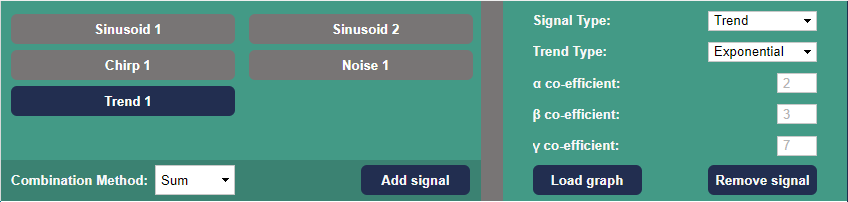
\includegraphics{img/configure_settings.PNG}
\caption{User configured signal settings}
\end{figure}

\newpage
\hypertarget{t7-display-of-individual-signals-and-stft-emd-analysis}{%
\subsection{T7: Display of individual signals and STFT / EMD
analysis}\label{t7-display-of-individual-signals-and-stft-emd-analysis}}

\hypertarget{member-responsible-saad-badshah}{%
\paragraph{Member Responsible: Saad
Badshah}\label{member-responsible-saad-badshah}}

\hypertarget{time-required-estimate-20-hours-2}{%
\paragraph{Time Required (Estimate): 20
hours}\label{time-required-estimate-20-hours-2}}

\hypertarget{depends-on-t1-t2-t3-t6-t8}{%
\paragraph{Depends on: T1, T2, T3, T6,
T8}\label{depends-on-t1-t2-t3-t6-t8}}

\hypertarget{description-5}{%
\paragraph{Description:}\label{description-5}}

As this system is intended to allow those with little prior knowledge on
signal analysis to further their understanding, time must be taken to
provide a high quality visual experience.

However, this task depends on the implementation of many other tasks,
and as such, only intial testing and decision of a JavaScript graphing
library will be done immediately.

Once the key dependancy, T6, has been completed, implementation can
begin of the actual display system for converting a
Python $\rightarrow$ Javascript array of time-points to a visual graph.
The other key dependancy for this task is T8, where the graph generated
must fit itself in well with the rest of the user interface, however
this is more in a non-functional stylistic manner rather than a
functional implementation manner.

A framework for completing this task is outlined below:
\begin{enumerate}
	\item Investigate and test which javascript graphing library will work well for our use case. Note that we intend to supply it only with a series of points and axis labels(i.e.~amplitude over time), and the graph must allow for pan and zoom over these time-points.
	\item Once key dependancies have been completed, implementation of reading Python global variables $\rightarrow$ graphing library in Javascript can be created.
	\item These graphs must then be placed where required in T8.
\end{enumerate}

\begin{figure}
\centering
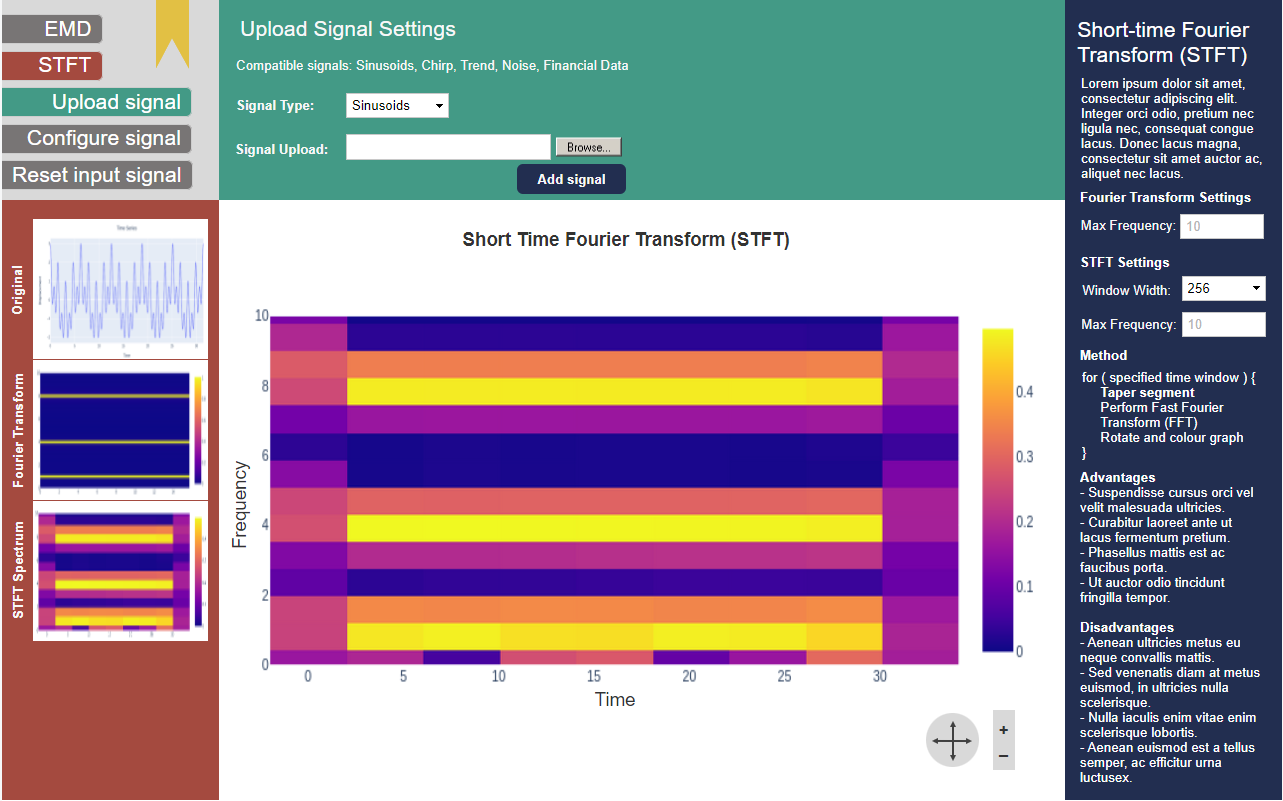
\includegraphics{img/STFT_upload.PNG}
\caption{Graph shown with pan and zoom controls}
\end{figure}

\newpage
\hypertarget{t8-design-and-implementation-of-user-interface}{%
\subsection{T8: Design and implementation of
User-Interface}\label{t8-design-and-implementation-of-user-interface}}

\hypertarget{member-responsible-abigail-rivera}{%
\paragraph{Member Responsible: Abigail
Rivera}\label{member-responsible-abigail-rivera}}

\hypertarget{time-required-estimate-20-hours-3}{%
\paragraph{Time Required (Estimate): 20
hours}\label{time-required-estimate-20-hours-3}}

\hypertarget{depends-on-t3-t6-1}{%
\paragraph{Depends on: T3, T6}\label{depends-on-t3-t6-1}}

\hypertarget{description-6}{%
\paragraph{Description:}\label{description-6}}

A clear consistent user interface (UI) is integral to the fulfilment of
the specification as the main use of this web application is educating
students with no prior knowledge of the subject matter i.e.~Time series
decomposition and allowing them to experiment with both methods. Within
this task the focus should be around the usefulness and effectiveness of
the UI and navigation through the application as an educational tool.
All controls, settings and access to graphs should be intuitive to use.

Steps for Completion: 

\begin{enumerate}
	\item Test wireframes designed and ensure they are possible to create within the chosen frontend technologies. Ensure frontend implementation will work well with chosen implementations for graphing animations, processing methods and signal manipulation.
	\item  Build a base frontend interface for both EMD and STFT methods based on wireframe designs, leaving placeholder sections for the generated graphs.
	\item Communicate with task leads on implementing the EMD, STFT methods as well as input signal manipulation for more detailed setting specifications and include this within the wireframe.
	\item Implement bookmarking functionality by adding flags onto URL which will allow the user to share their configuration.
	\item Ensure all class and id names follow the same convention and are consistent with other parts of the application.
\end{enumerate}

\begin{figure}
\centering
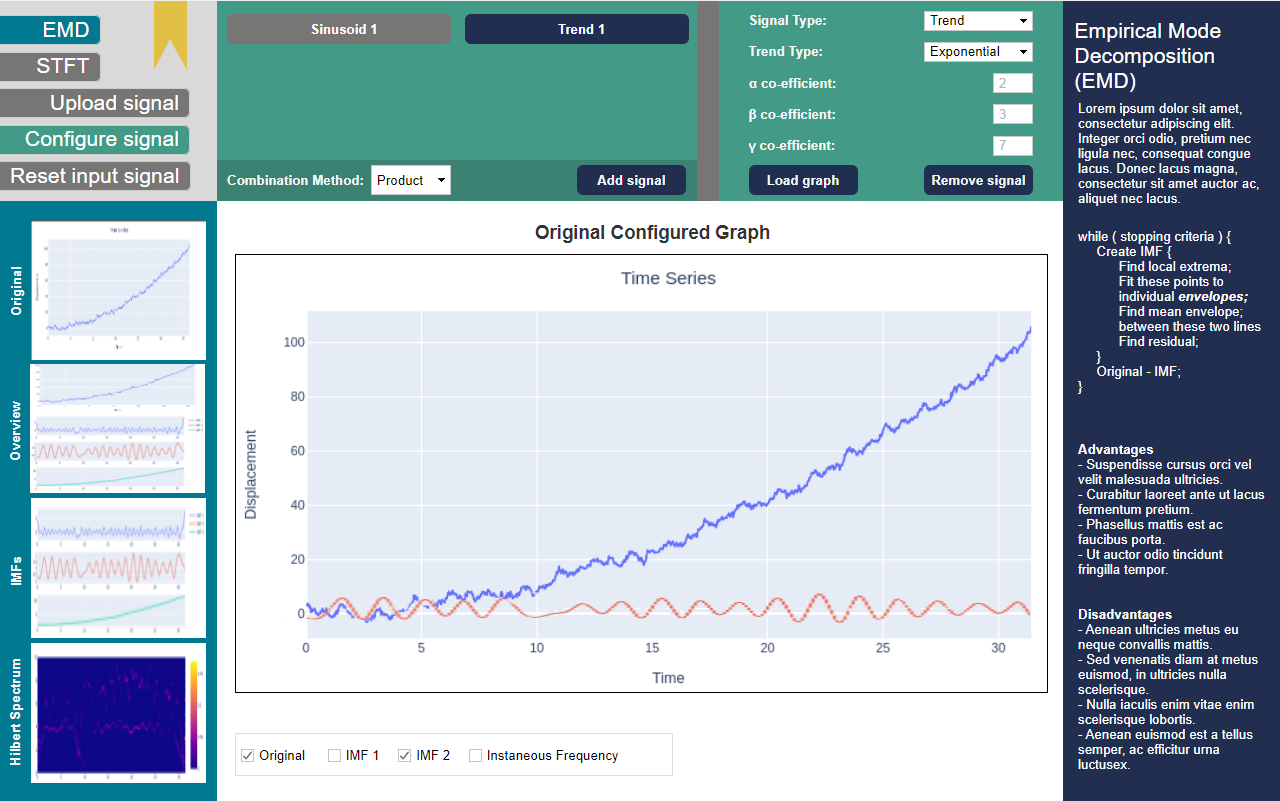
\includegraphics{img/EMD_multiple_product_signal.PNG}
\caption{EMD approach applied to user configured combined signal by
product}
\end{figure}

\begin{figure}
\centering
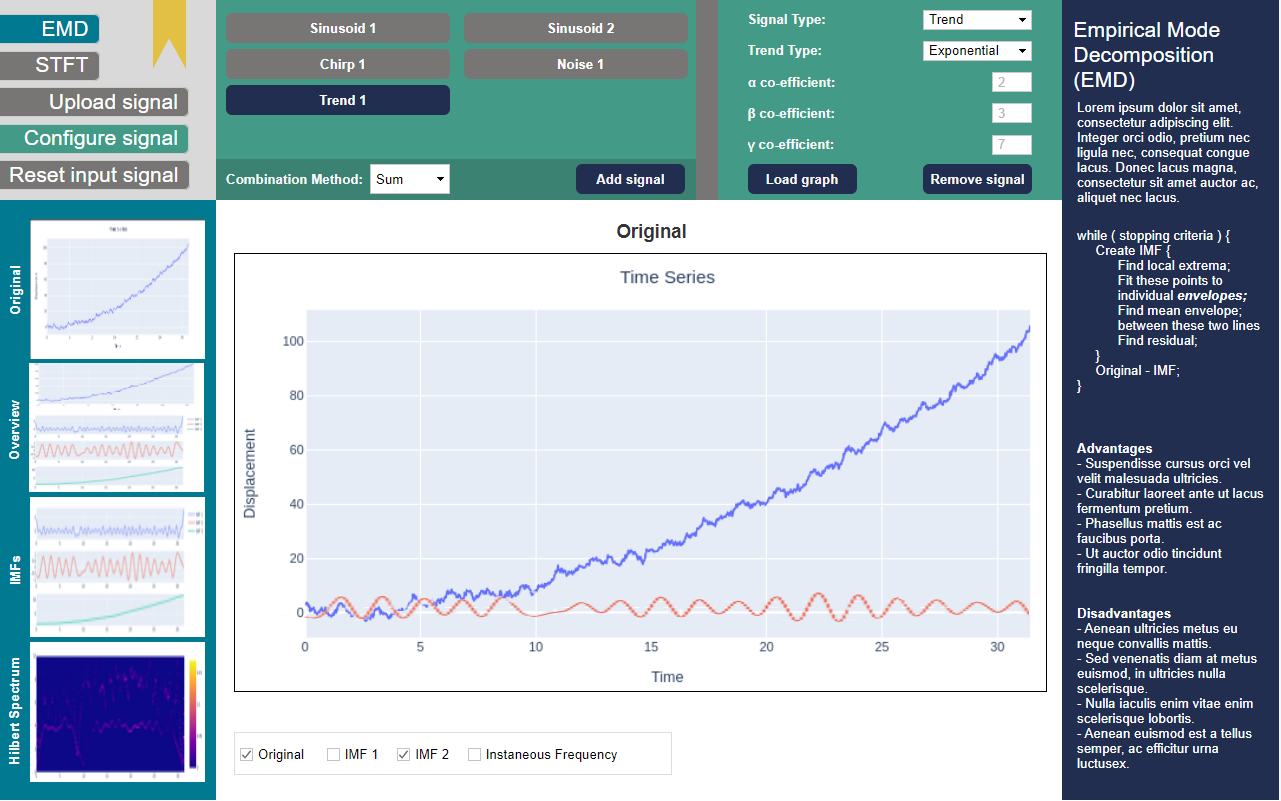
\includegraphics{img/EMD_multiple_sum_signal.PNG}
\caption{EMD approach applied to user configured combined signal by sum}
\end{figure}

\begin{figure}
\centering
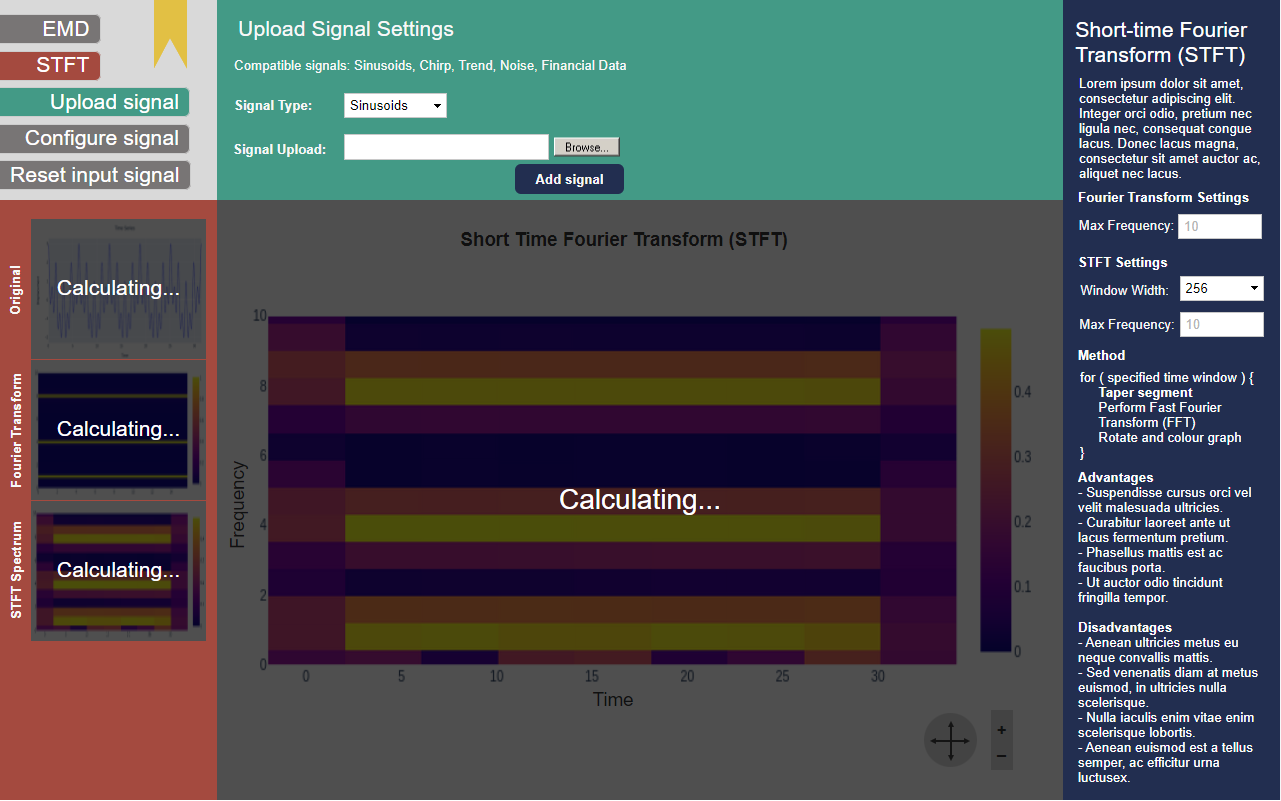
\includegraphics{img/Loading_graphs.PNG}
\caption{Loading overlay triggered with changes in signal or method
chosen}
\end{figure}

\begin{figure}
\centering
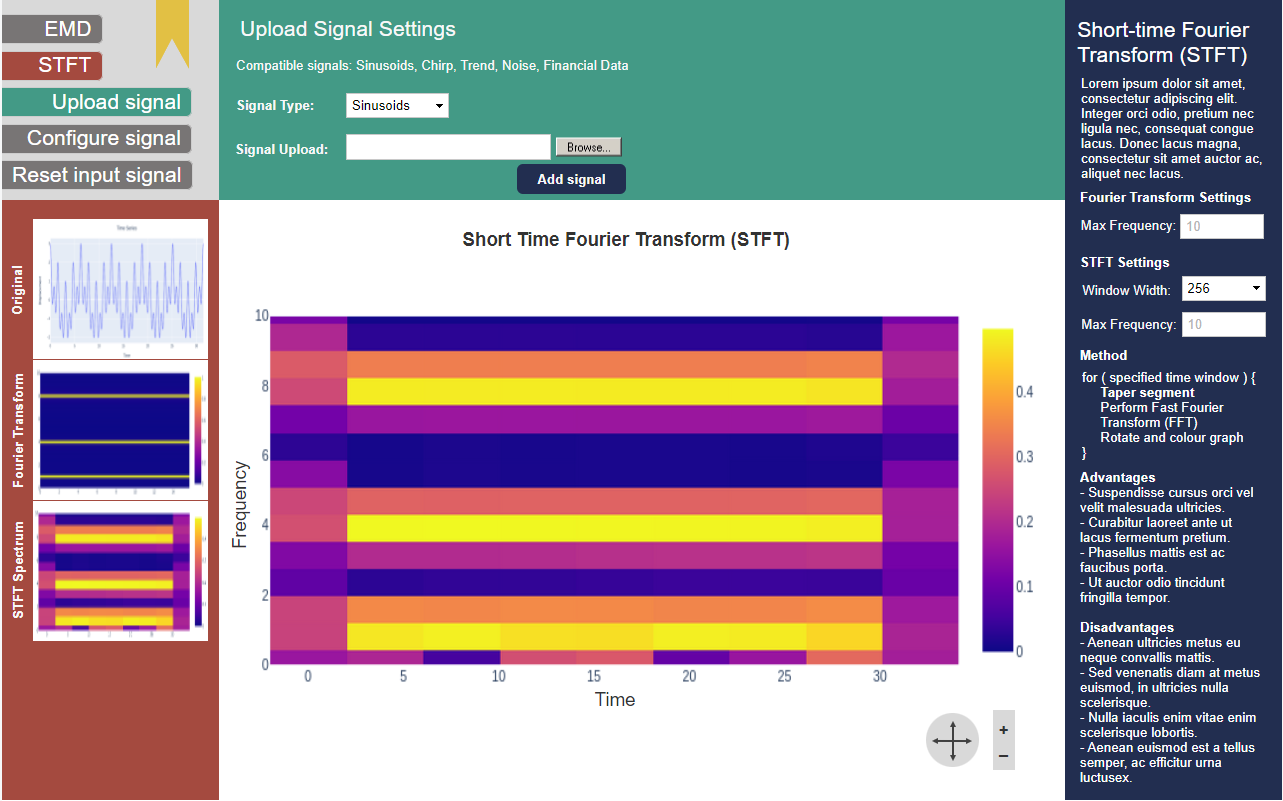
\includegraphics{img/STFT_upload.PNG}
\caption{STFT approach applied to uploaded signal}
\end{figure}

\newpage
\hypertarget{t9-integration-testing}{%
\subsection{T9: Integration Testing}\label{t9-integration-testing}}

\hypertarget{member-responsible-sebastian}{%
\paragraph{Member Responsible:
Sebastian}\label{member-responsible-sebastian}}

\hypertarget{time-required-estimate-10-hours}{%
\paragraph{Time Required (Estimate): 10 hours}\label{time-required-estimate-10-hours}}

\hypertarget{depends-on-all}{%
\paragraph{Depends on: All}\label{depends-on-all}}

\hypertarget{description-7}{%
\paragraph{Description:}\label{description-7}}

All software modules that pass unit testing will be subjected to
integration testing to ensure the application works as a whole.

Steps for completion:
\begin{enumerate}
	\item Identify methodology or framework to be used for integration testing, ensure this is compatible with unit testing process.
	\item Iteratively include all modules as they are completed and updated into the integration testing and provide feedback in a timely manner to the team with any failures identified and possible solutions if applicable.
\end{enumerate}

\newpage
\hypertarget{t10-creation-of-a-tutorial}{%
\subsection{T10: Creation of a
Tutorial}\label{t10-creation-of-a-tutorial}}

\hypertarget{member-responsible-callum-stewart-1}{%
\paragraph{Member Responsible: Callum
Stewart}\label{member-responsible-callum-stewart-1}}

\hypertarget{time-required-estimate-20-hours-4}{%
\paragraph{Time Required (Estimate): 20
hours}\label{time-required-estimate-20-hours-4}}

\hypertarget{depends-on-t7-t8}{%
\paragraph{Depends on: T7, T8}\label{depends-on-t7-t8}}

\hypertarget{description-8}{%
\paragraph{Description:}\label{description-8}}

A tutorial supplemented by the use of designed web app is crucial to
fulfilling Deliverable 3. This will involve writing a clear and concise
technical article geared toward an audience with a CS background and no
prior knowledge of EMD or STFT. The main objective of this task is to
allow the user to learn about both methods namely their advantages and
disadvantages in order to compare the approaches.

Steps for Completion 
\begin{enumerate}
	\item Gather useful external materials (peer-reviewed papers, video links) that may be linked within the tutorial paper when gaining a thorough understanding of each method.
	\item Create a brief introduction explaining the methods and steps taken to implement each method, although these should also be available in the application itself.
	\item Collate main advantages and disadvantages of these methods in order to create examples to demonstrate and highlight these.
	\item Outline a guide with screenshots and descriptions to using the application including importing signals, combining signals, configuring method settings, applying each method, navigating different graphs produced, overlaying graphs on same time axis and bookmarking.
	\item Create tasks to work through that demonstrate the various advantages and disadvantages of each method using various different signal types.
\end{enumerate}

\newpage
\hypertarget{t11-continuous-risk-management}{%
\subsection{T11: Continuous Risk
Management}\label{t11-continuous-risk-management}}

\hypertarget{member-responsible-daniel}{%
\paragraph{Member Responsible: Daniel}\label{member-responsible-daniel}}

\hypertarget{time-required-estimate-50}{%
\paragraph{Time Required (Estimate):
50}\label{time-required-estimate-50}}

\hypertarget{depends-on-all-1}{%
\paragraph{Depends on: All}\label{depends-on-all-1}}

\hypertarget{description-9}{%
\paragraph{Description:}\label{description-9}}

Managing risk within this project will be handled through an iterative
proccess of identifying, preventing and mitigating any known risks. This
will be done each week to ensure all critical failures are avoided or
mitigated early on. Through the D1 deliverable a risk table has been
created with existing risks and will be updated by the task leader with
feedback from the rest of the group when required.

\newpage
\hypertarget{t12-demo-presentation}{%
\subsection{T12: Demo Presentation}\label{t12-demo-presentation}}

\hypertarget{member-responsible-saad}{%
\paragraph{Member Responsible: Saad}\label{member-responsible-saad}}

\hypertarget{time-required-estimate-4-hours}{%
\paragraph{Time Required (Estimate): 4
hours}\label{time-required-estimate-4-hours}}

\hypertarget{depends-on-all-2}{%
\paragraph{Depends on: All}\label{depends-on-all-2}}

\hypertarget{description-10}{%
\paragraph{Description:}\label{description-10}}

After developing a project its very important to have a presentation for
the users that can watch it and understand the full functionality of the
application. After the completion of this web application, all the
members of the team will make a seminar style project demonstration and
a presentation. The steps involved in creating the demo are listed as
follows:

Steps for Demonstration:
\begin{enumerate}
	\item Each individual responsible for a piece of functionality they have been working on will capture a short screen recording of the working functionality they have developed.
	\item The team should then make a powerpoint presentation which includes slides on introduction to the project, The background information, Architecture of the application, Justification for the technologies used in development and the must have functional requirements, and the planning process which went behind the decisions made to implement the key functionality.  Class diagrams, flow charts etc can be added to explain the architecture in more detail.
	\item The tasks that were assigned will be discussed by each individual that was responsible for the task, the screen recording captured in step 1 should be played and the person who developed it should discuss it in further detail going in detail about how the flow of the functionality works.
	\item Future improvements section should be included which discusses the future functionality that can be added to the application to make it more efficent and even perform more detailed analysis and any future functionality that we might want to add.
	\item In the end a conclusion section should be included which discussed the key take aways from this project.
\end{enumerate}

\newpage
\hypertarget{t13-creation-of-the-design-manual}{%
\subsection{T13: Creation of the design
manual}\label{t13-creation-of-the-design-manual}}

\hypertarget{member-responsible-daniel-1}{%
\paragraph{Member Responsible:
Daniel}\label{member-responsible-daniel-1}}

\hypertarget{time-required-estimate-5-hours-1}{%
\paragraph{Time Required (Estimate): 5
hours}\label{time-required-estimate-5-hours-1}}

\hypertarget{depends-on-all-3}{%
\paragraph{Depends on: All}\label{depends-on-all-3}}

\hypertarget{description-11}{%
\paragraph{Description:}\label{description-11}}

As part of the D2 deliverable, a design manual needs to be created that
includes a top-level design and enough detail to allow reuse and
modification for other students with similar backgrounds without prior
knowledge or communication about the application.

Steps for completion: 

\begin{enumerate}
	\item Identify and document all technologies and libraries used with links where appropriate.
	\item Include documentation of how each software module was implemented and any critical notes that may affect further modification.
	\item Design a top-level diagram of how each part of the system works together.
\end{enumerate}

\newpage
\hypertarget{risk-analysis}{%
\section{Risk Analysis}\label{risk-analysis}}

In this section we will outline any possible risk that could slow down
the project in any way and create a plan of action to minimise the
effect any unexpected circumstances have on it.

This section will be split into 4 tables: - General Riks - Technical
Risks - Actions to Reduce Severity - Completed Actions

The `General Risks' section outlines potential risks to the project
which cannot be categorised as `technical'. We describe the possible
risks, give them a severity and the chance of the risk occurring. A
concise mitigation plan is also written up to give our team a clear plan
that will help resolve any problems caused by the risk.

In `Technical Risks' we focus on the technical aspect of the project. We
outline the same information as in the `General Risks': a description,
severity, chance of occuring and a mitigation plan, as well as a risk ID
that is used in the later tables to identify which action correlates to
which risk.

The severity and chance of occuring in the `General Risks' and
`Technical Risks' tables can be either: Low, Medium or High. With these
values we order the tables so the risks that have the possibility to
cause the biggest delays to the project are at the top, this will help
us later when defining possible actions to reduce risks as the most
severe risks should be tackled first..

In `Actions to Reduce Severity' we outline actions that should be done
to reduce either the severity or the chance of the risk occurring for a
particular risk. The table outlines which technical risk will be
affected, a person responsible for completing this action and a brief
description of the task to be completed. The actions were created in the
order of the risks in the `Technical Risks' table since the most severe
risks are at the top of the table.

The final table `Completed Actions' is used to keep a record of what
actions have been completed and how they affected the project risks. The
table consists of the risk number, the person responsible for completing
the task and how it affected the severity and chance of happening.

\begin{center}\rule{0.5\linewidth}{0.5pt}\end{center}

\hypertarget{general-risks}{%
\subsection{General Risks}\label{general-risks}}

\begin{longtable}[]{@{}
  >{\raggedright\arraybackslash}p{(\columnwidth - 6\tabcolsep) * \real{0.1875}}
  >{\centering\arraybackslash}p{(\columnwidth - 6\tabcolsep) * \real{0.3125}}
  >{\centering\arraybackslash}p{(\columnwidth - 6\tabcolsep) * \real{0.3125}}
  >{\raggedright\arraybackslash}p{(\columnwidth - 6\tabcolsep) * \real{0.1875}}@{}}
\toprule
\begin{minipage}[b]{\linewidth}\raggedright
Risk Description
\end{minipage} & \begin{minipage}[b]{\linewidth}\centering
Severity
\end{minipage} & \begin{minipage}[b]{\linewidth}\centering
Chance of Occuring
\end{minipage} & \begin{minipage}[b]{\linewidth}\raggedright
Mitigation Plan
\end{minipage} \\
\midrule
\endhead
Group members not attending a group meeting unexpectedly. & Medium & Low
& Project Lead will take over the speaking points of the missing group
member. Also if any task allocations are made during a meeting the group
member will have no input over their task (As long as they are allocated
reasonably) \\
Group members unable to complete their tasks due to being ill. & Medium
& Medium & As soon as we are notified that a group member is unable to
complete their current task due to being ill we will have to evaluate
what work has been done this week and allocate the incomplete task to
group members with the most available time. \\
Group members not communicating with the rest of the team. & Medium &
Low & If a group member goes silent their work will have to be
redistributed among the rest of the team for the time they are not
responding or until the rest of the project as deadlines still have to
be met. \\
Data being lost during the project. & High & Low & Depending on how far
into the project we are, restarting the project might be an option but
if this would happen near the deadline the project would have to be
terminated. To keep the chances as low as possible of any data being
lost, all project files, code and report are uploaded to GitLab.
Additionally some group members will regularly download a backup of the
GitLab repository. \\
Gantt chart deadlines not being met. & High & Medium & If deadlines are
being missed we will have to re-evaluate the requirements and focus on
the main functionality outlined by `Must Have' in the requirements,
while decreasing the priority on the `Should Have' and `Could Have'. \\
Group members disagrees with a project decision & Medium & Low & If only
one or two members disagree with a decision it will ultimately be our
project lead's choice, if the group member still disagrees they can
escalate the problem to the project supervisor. \\
Group members having too much work allocated & High & Medium & Each
group member is responsible for their own allocated tasks, if they seem
that they are falling behind with too much work they are responsible to
ask the rest of the team to help with completing their task. \\
Group members having too little work allocated & Medium & Medium & If a
group member completes their tasks ahead of schedule they should message
the team and offer their help with other sections currently being worked
on. \\
The timing of the planned work not being accurate & Low & Medium & If
during development there are clear misjudgments of the time taken to
complete a task we will adjust the time for the tasks that have not yet
been finished to create a clearer image of how long the tasks will
take. \\
\bottomrule
\end{longtable}

\hypertarget{technical-risks}{%
\subsection{Technical Risks}\label{technical-risks}}

\begin{longtable}[]{@{}
  >{\centering\arraybackslash}p{(\columnwidth - 8\tabcolsep) * \real{0.2174}}
  >{\raggedright\arraybackslash}p{(\columnwidth - 8\tabcolsep) * \real{0.1304}}
  >{\centering\arraybackslash}p{(\columnwidth - 8\tabcolsep) * \real{0.2174}}
  >{\centering\arraybackslash}p{(\columnwidth - 8\tabcolsep) * \real{0.2174}}
  >{\raggedright\arraybackslash}p{(\columnwidth - 8\tabcolsep) * \real{0.2174}}@{}}
\toprule
\begin{minipage}[b]{\linewidth}\centering
Risk Number
\end{minipage} & \begin{minipage}[b]{\linewidth}\raggedright
Risk Description
\end{minipage} & \begin{minipage}[b]{\linewidth}\centering
Severity
\end{minipage} & \begin{minipage}[b]{\linewidth}\centering
Chance Of Occuring
\end{minipage} & \begin{minipage}[b]{\linewidth}\raggedright
Mitigation Plan
\end{minipage} \\
\midrule
\endhead
1 & The EMD or STFT python libraries break when running in the browser
via \passthrough{\lstinline!Pyodide!}. & Medium & Medium & Depending on
the cause of code breaking we will either find alternative libraries for
EMD or STFT if they are the cause of the problems, or we will need to
port Python code to JavaScript if `Pyodide' is the problem. \\
2 & EMD or STFT libraries braking during runtime. Very unique edge cases
can cause the code to break but the majority must be fully working.
Possible extra problems caused if we are forced to translate parts of
code from Python to JavaScript. & Medium & High & If the current
libraries are causing too many problems to continue, alternative
libraries will have to be found to replace the currently used ones. \\
3 & Initial functional requirements not fully planned out. & High &
Medium & If during development we find a part of the requirements to not
be fully explained in the functional requirements we will set up a short
meeting to create a plan for the missing requirements and assign tasks
accordingly. \\
4 & Support for EMD or STFT in JavaScript might not exist and may need
to be ported from Python. & High & Medium & Since our plan is to execute
Python code in the browser this has a low chance of being a risk but we
may need to port over Python code to JavaScript. \\
5 & System memory problems during the runtime of Python code in the
browser. First tests of running code in the browser identified this as a
possibility. & Medium & Medium & We will need to find the source of the
problem and either fix the code ourselves or find better and more
performant libraries that accomplish the same task. \\
6 & Problems with GitLab collaboration. & Medium & Medium & As GitLab is
a requirement in this project, GitLab breaking would be a unique
circumstance that would need to be resolved with the project
supervisor. \\
7 & Not fully understanding the mathematics behind EMD or STFT. & Medium
& Low & Meet up with Cole if possible to get clarification on parts of
the mathematics that we do not understand. \\
8 & Concurrency issues in JavaScript. In testing we found that using
Python in the browser via \passthrough{\lstinline!Pyodide!} runs
everything on the main thread and the web page becomes unresponsive
while running code, so concurrency will need to be added for a smoother
experience. & Low & Medium & If during development we are unable to make
the application concurrent, we will just have to run the application on
a single thread which isn't a big problem as having the application run
faster is just a `Nice to have' feature. Will just need to add a warning
for the user to inform them that the application might appear frozen at
times. \\
9 & User interface of the front end missing features or badly designed.
& Medium & Low & We will need to sketch up new interface mockups and
focus on adding features we have missed in the planning stage or were
badly designed. \\
10 & Requirement analysis document missing sections, incomplete sections
or sections aren't up to the specifications. & Medium & Low & If any
requirements are found to be missing during development we will need to
organise a meeting to create plans for the missing requirements and
allocate the tasks. \\
\bottomrule
\end{longtable}

\newpage
\hypertarget{current-actions-to-reduce-severity}{%
\subsection{Current Actions to Reduce
Severity}\label{current-actions-to-reduce-severity}}

\begin{longtable}[]{@{}
  >{\centering\arraybackslash}p{(\columnwidth - 4\tabcolsep) * \real{0.3846}}
  >{\centering\arraybackslash}p{(\columnwidth - 4\tabcolsep) * \real{0.3846}}
  >{\raggedright\arraybackslash}p{(\columnwidth - 4\tabcolsep) * \real{0.2308}}@{}}
\toprule
\begin{minipage}[b]{\linewidth}\centering
Risk Number
\end{minipage} & \begin{minipage}[b]{\linewidth}\centering
Person Responsible
\end{minipage} & \begin{minipage}[b]{\linewidth}\raggedright
Possible Action to Reduce Severity
\end{minipage} \\
\midrule
\endhead
2 & Callum & Create unit tests to check how robust the EMD and STFT
libraries are, if any problems are found we will try to fix the code
that's affecting it or if that is unfeasible we will notify the user of
the limitations if there are any.Run extra tests in a
\passthrough{\lstinline!Pyodide!} environment to further test the
robustness of both the code and the Python code running in browser. \\
2 & Saad & Find alternative libraries to the currently used ones. If any
problems occur with the current libraries, almost no downtime will be
required to replace them. \\
3 & Saad & If possible meet up with Cole and present the current
requirements and get feedback from him and make any change to the
requirements that he may suggest. \\
6 & Sebastian & Have a session with the entire team to make sure every
team member fully understands how collaboration in GitLab works. \\
9 & Abigail & A meeting with Cole would be ideal as he will know best
what the users would look for in the front end, possibly discuss this in
the same meeting as the requirements. \\
6 & Sebastian & Create backups locally on their personal computer just
in case a problem with GitLab occurs. \\
4 & Daniel & Research the currently available EMD and STFT JavaScript
libraries and see if they provide all the functionality we require for
the project. \\
5 \& 8 & Bruce & Both these risks are related to `Pyodide', a simple
test environment will need to be created to test web workers and that
the solution will have no problems with running out of system memory. \\
\bottomrule
\end{longtable}

\newpage
\hypertarget{completed-actions}{%
\subsection{Completed Actions}\label{completed-actions}}

\begin{longtable}[]{@{}
  >{\centering\arraybackslash}p{(\columnwidth - 4\tabcolsep) * \real{0.3846}}
  >{\centering\arraybackslash}p{(\columnwidth - 4\tabcolsep) * \real{0.3846}}
  >{\raggedright\arraybackslash}p{(\columnwidth - 4\tabcolsep) * \real{0.2308}}@{}}
\toprule
\begin{minipage}[b]{\linewidth}\centering
Risk Number
\end{minipage} & \begin{minipage}[b]{\linewidth}\centering
Person Responsible
\end{minipage} & \begin{minipage}[b]{\linewidth}\raggedright
Action and effect on risk
\end{minipage} \\
\midrule
\endhead
10 & Daniel & As a team we discussed the state of the document,
specifically the requirement to ensure there are no specifications that
we have not planned for.Chance of Occuring: Medium -\textgreater{}
Low \\
7 & Callum & Do background research on EMD and STFT to fully understand
all the specification outline in the project specification.Chance of
Occuring: Medium -\textgreater{} Low \\
1 & Bruce & Create a test environment to test running Python code in
browser via \passthrough{\lstinline!Pyodide!}, if unsuccessful, test the
other options discussed in the first meeting.Chance of Occuring: High
-\textgreater{} MediumSeverity: High -\textgreater{} Medium \\
\bottomrule
\end{longtable}

\newpage
\hypertarget{software-integration-plan}{%
\section{Software Integration Plan}\label{software-integration-plan}}

Care must be taken during planning to ensure that each of the developed
software systems integrate with one another seamlessly. To do this, a
plan must be made that takes into account each tasks dependencies on
others, and organises which order software modules must be combined for
incremental systems testing.

The implementation side of the project can be split into two key areas.
The first is our Python ``backend'' (by backend, we mean a full CPython
WebAssembly implementation running \textbf{in browser}) which performs
all our numerical calculations and analysis, such as STFT, EMD, and
signal generation/combining. The second is our JavaScript/html
``frontend'', which handles visualisation of the returned data sets from
the Python backend, alongside handing data transfer from the user to the
backend.

Due to the nature of the Python backend scripting and frontend
development, these developments can be parallelised.

However, an agreement must be made in the order of arguments being
passed between the frontend interface and the backend. These can be
summarised below:

\begin{itemize}
\tightlist
\item
  When ``add signal'' button is clicked:

  \begin{itemize}
  \tightlist
  \item
    Signal type + signal parameters must be passed to the backend from
    user interface input parameters (plus any summing information for a
    combined signal).
  \item
    Backend must return an array of time-points representing the signal
    (plus any combined signal).
  \item
    Frontend should handle the array of time-points and display them on
    an interactive graph.
  \end{itemize}
\end{itemize}

Note that from the above summary, there is two discrete information
passes. When the frontend sends the user input parameters to the
backend, and when the backend returns the array of time points. Due to
the implementation of backend\textless-\textgreater front end that we
are using, the key thing to take into account is data types when
converting from Python to Javascript, for example, numpy arrays may
convert to difficult to use objects in Javascript. Testing of this must
be performed early to ensure later development can flow easily.

A second data passing scenario is summarised below:

\begin{itemize}
\tightlist
\item
  When ``analyse signal'' is initiated:

  \begin{itemize}
  \tightlist
  \item
    Type of analysis to perform + any parameters must be passed to the
    backend from the user interface.
  \item
    The backend already knows which signals have been generated
    previously (or uploaded signals), alongside their combined signal.
  \item
    Specified analysis type must be performed by the backend, returning
    the appropriate data depending on the analysis type (e.g.~EMD
    -\textgreater{} IMF's\ldots).
  \end{itemize}
\end{itemize}

Note that here, the data that is being passed back may be more complex
than simple 1D arrays as before with the time-point signal arrays.

Using the two examples listed above, we can see that the Python backend
is acting similar to a RESTful API, however with statefulness (as the
Python backend is only serving one user on their own browser, we can
save large data back and forth by storing the state of the signals
generated).

What this means is we can create the Python signal generating code,
signal combining, EMD analysis, STFT analysis, as separate Python
modules that all can communicated with from Javascript, and all can
communicate to store their state with a memory module (or more simply,
organised Python globals).

These modules in theory can be developed independently from each other,
however they must follow the agreements made previously on which data
and in what order it will be sent.

Following the above theory, the following plan is created:

\begin{itemize}
\tightlist
\item
  Development of the frontend interface bar signal
  graphing/visualisation shall begin immediately.
\item
  Development of signal generation in Python can begin immediately, with
  the agreement of which input parameters shall be sent through
  Javascript to the backend. These signals generated must be stored in a
  Python global scope, in a format that is reusable in Python and
  Javascript (e.g.~1D array)
\item
  Development of the signal combination can begin once the signal
  generation code is able to save data to the Python global scope. This
  combined signal will also be stored in a Python global scope.
\item
  Development of the STFT and EMD algorithms can begin once the signal
  combination is able to save data to the Python global scope (accessing
  the combined data signal).
\item
  Development of the user-uploading data can begin once the signal
  generation Python module is complete. This ensures that the uploaded
  data module will have to use the agreed upon combined signal storing
  method, and EMD/STFT will be able to access the user uploaded data as
  if it was generated with our system.
\item
  Development of the graphing system can begin once signal generation is
  able to return data from Python. This may not include all signal
  types, however once one signal type is correctly being stored and
  returned, it can be used as an example of how all other signals will
  be returned from Python to be displayed on the frontend.
\item
  Development of the tutorial can begin once the graphing system
  alongside frontend interface are near completion.
\end{itemize}

Due to the nature of the Python modules, unit testing will be able to be
performed on each component individually, alongside following the plan
above will aid with knowing when each part of the system can join as
part of the system integration tests.

\newpage
\hypertarget{gantt-chart}{%
\section{Gantt Chart}\label{gantt-chart}}

\begin{figure}
\centering
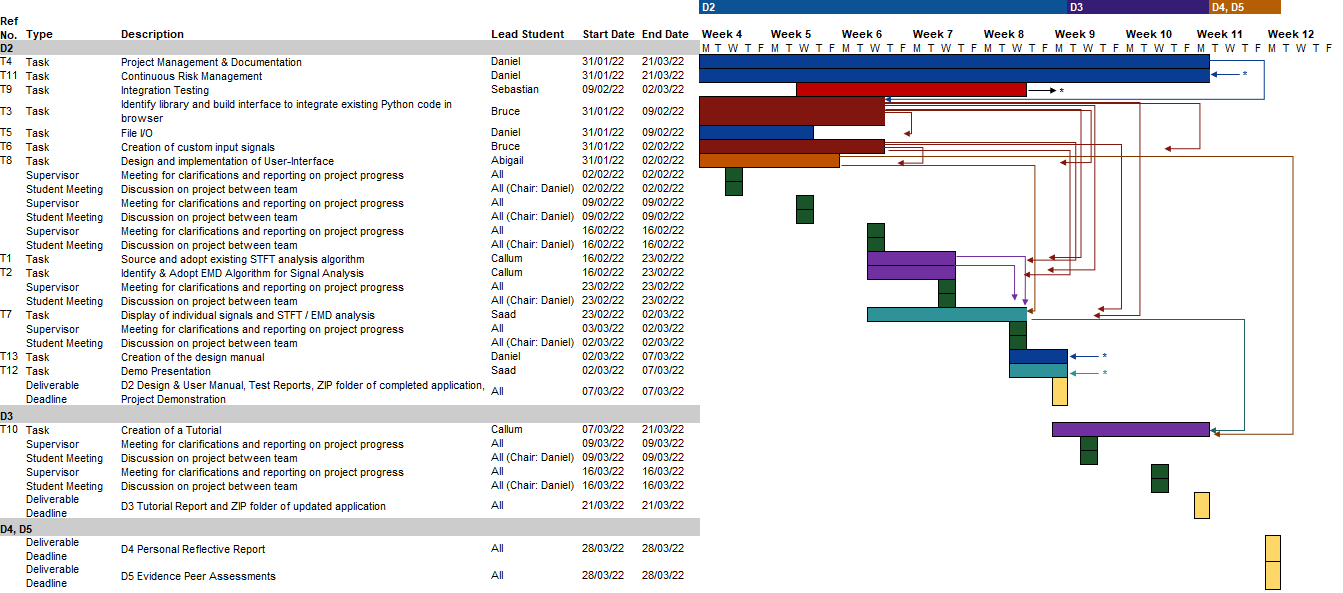
\includegraphics{img/GanttChartFinal.PNG}
\caption{Whole Project Gantt Chart}
\end{figure}

Note.\\
\begin{itemize}
	\item ``* $\leftarrow$'' denotes that this task is dependant on all other tasks 
	\item ``$\rightarrow$ *'' denotes that all tasks are dependent on this task
\end{itemize}

\newpage
\hypertarget{gantt-asdf-chart}{%
\section{Table of Responsiblities}\label{gantt-chart-asdf}}

The table below outlines how the reponsiblities in the team are distributed
using the RACI model with the acronyms being explained in the key below.

\begin{longtable}[]{@{}
  >{\centering\arraybackslash}p{(\columnwidth - 4\tabcolsep) * \real{0.3846}}
  >{\raggedright\arraybackslash}p{(\columnwidth - 4\tabcolsep) * \real{0.2308}}
  >{\centering\arraybackslash}p{(\columnwidth - 4\tabcolsep) * \real{0.3846}}@{}}
\toprule
\begin{minipage}[b]{\linewidth}\centering
Acronym
\end{minipage} & \begin{minipage}[b]{\linewidth}\raggedright
Role
\end{minipage} & \begin{minipage}[b]{\linewidth}\centering
Description
\end{minipage} \\
\midrule
\endhead
R & Responsible & Team members who work to complete the task. \\
A & Accountable & Task leader i.e.~the one answerable for the completion
of the task. \\
C & Consulted & Team members who should be contacted and dicuss matters
relating to the task. \\
I & Informed & Team members who should be informed of task progress
usually on completion of a task. \\
\bottomrule
\end{longtable}

\begin{longtable}[]{@{}
  >{\centering\arraybackslash}p{(\columnwidth - 14\tabcolsep) * \real{0.1471}}
  >{\raggedright\arraybackslash}p{(\columnwidth - 14\tabcolsep) * \real{0.0882}}
  >{\centering\arraybackslash}p{(\columnwidth - 14\tabcolsep) * \real{0.1471}}
  >{\centering\arraybackslash}p{(\columnwidth - 14\tabcolsep) * \real{0.1471}}
  >{\raggedright\arraybackslash}p{(\columnwidth - 14\tabcolsep) * \real{0.0882}}
  >{\centering\arraybackslash}p{(\columnwidth - 14\tabcolsep) * \real{0.1471}}
  >{\raggedright\arraybackslash}p{(\columnwidth - 14\tabcolsep) * \real{0.0882}}
  >{\centering\arraybackslash}p{(\columnwidth - 14\tabcolsep) * \real{0.1471}}@{}}
\toprule
\begin{minipage}[b]{\linewidth}\centering
Task Number
\end{minipage} & \begin{minipage}[b]{\linewidth}\raggedright
Task Description
\end{minipage} & \begin{minipage}[b]{\linewidth}\centering
Bruce
\end{minipage} & \begin{minipage}[b]{\linewidth}\centering
Callum
\end{minipage} & \begin{minipage}[b]{\linewidth}\raggedright
Saad
\end{minipage} & \begin{minipage}[b]{\linewidth}\centering
Sebastian
\end{minipage} & \begin{minipage}[b]{\linewidth}\raggedright
Abigail
\end{minipage} & \begin{minipage}[b]{\linewidth}\centering
Daniel
\end{minipage} \\
\midrule
\endhead
T1 & Source and adopt existing STFT analysis algorithm & C & A & C & I &
I & C \\
T2 & Identify \& Adopt EMD Algorithm for Signal Analysis & C & A & C & I
& I & C \\
T3 & Identify library and build interface to integrate existing Python
code in browser & A & C & I & R & C & C \\
T4 & Project Management \& Documentation & I & R & C & I & R & A \\
T5 & File I/O & C & I & I & I & C & A \\
T6 & Creation of custom input signals & A & C & R & I & C & I \\
T7 & Display of individual signals and STFT / EMD analysis & R & C & A &
I & C & C \\
T8 & Design and implementation of User-Interface & C & C & C & I & A &
C \\
T9 & Integration Testing & C & C & C & A & C & C \\
T10 & Creation of a Tutorial & I & A & C & C & R & I \\
T11 & Continuous Risk Management & C,R & C,R & C,R & C,R & C,R & A \\
T12 & Demo Presentation & C,R & C,R & A,R & C,R & C,R & C,R \\
T13 & Creation of the design manual & C & C & I & I & C & A \\
\bottomrule
\end{longtable}

\newpage
\hypertarget{requirements-traceability-matrix}{%
\section{Requirements Traceability
Matrix}\label{requirements-traceability-matrix}}

\begin{longtable}[]{@{}
  >{\raggedright\arraybackslash}p{(\columnwidth - 4\tabcolsep) * \real{0.2857}}
  >{\centering\arraybackslash}p{(\columnwidth - 4\tabcolsep) * \real{0.4286}}
  >{\raggedleft\arraybackslash}p{(\columnwidth - 4\tabcolsep) * \real{0.2857}}@{}}
\toprule
\begin{minipage}[b]{\linewidth}\raggedright
ID
\end{minipage} & \begin{minipage}[b]{\linewidth}\centering
Requirement Description
\end{minipage} & \begin{minipage}[b]{\linewidth}\raggedleft
Task ID
\end{minipage} \\
\midrule
\endhead
FR-1-1 & The application must support Short-Time Fourier Transform
(STFT) time series analysis on input signal data. & T1 \\
FR-1-2 & The application must support Empirical Mode Decomposition (EMD)
time series analysis on input signal data and export the resultant IMFs
for use in other components of the application. & T2 \\
FR-1-3 & The application must support the deconstruction of given,
identifiable signal data into its respective functional components. I.e.
Deconstruct periodical sinusoidal signal data via STFT and display its
extracted frequencies in a spectragram. & T2 \\
FR-2-1 & The application must plot the output of a signal analysis
request (STFT, EMD) on given input data visually in a graph embedded in
the webpage. & T7 \\
FR-2-2 & The application must support simultaneously displaying the
original, unaltered signal data and the extracted components on a common
time base (i.e.~over a period of 10 seconds) in a graph embedded in the
webpage. & T7 \\
FR-2-3 & The application must support simultaneously displaying the
instantaneous frequencies of the original components alongside the IMF
and STFT estimates in a graph embedded in the webpage. & T7 \\
FR-2-4 & The application must support `bookmarking' functionality;
allowing users to share their configurations and parameters for signal
analysis. & T8 \\
FR-2-5 & The application must explain the advantages and disadvantages
between STFT and EMD signal analysis. & T10 \\
FR-2-6 & The application should display animations showcasing the
differences in techniques and behaviours between EMD and STFT analysis.
& T10 \\
FR-2-7 & The application should allow the user to generate custom signal
data from a set of pre-defined types for processing. & T6 \\
FR -3-1 & The application must be extensively tested via unit and
integration testing to verify individual components behave predictably
and correctly, and multiple components working in conjunction behave
reliably and deliver the expected result. & T9 \\
FR -3-2 & The application must support raw signal data to be uploaded
for processing by an end user, and not just rely on pre-generated
examples. & T5 \\
NFR 1-1 & The web application will be easy to use for users. & T8 \\
NFR 1-2 & The application must have predefined signal types, which the
user can choose from through a drop-down list. & T6 \\
NFR 1-3 & The web application will have an online tutorial embedded for
the users to see and learn about the advantages and disadvantages of EMD
and STFT. & T10 \\
NFR 1-4 & Allow users to save data visualisations. & T8 \\
NFR 2-1 & The web application will have no back-end, all of the
functionality will be implemented on the front-end. & T3 \\
NFR 2-1 & The application will have low latency, the application will be
effiecient in regards to the overhead of the data visualisation. & T7 \\
NFR 2-1 & The application will allow different kinds of data input by
the user. It will support data in formats such as CSV. & T5 \\
NFR 2-1 & The application will be efficent with the usage of the memory,
to allow smooth animations of the data visualisation and avoid memory
problems. & T7 \\
NFR 3-1 & The web application will be compatibility across multiple
platforms (FireFox, Chrome). & T8 \\
NFR 3-2 & The web application will be able to handle stress, it will be
stress tested to prevent any glitching or any unexpected events to
occur. & T9 \\
NFR 3-3 & The application will not be tested or designed for use on
Mobile devices. & T8 \\
\bottomrule
\end{longtable}

\end{document}
